\documentclass[12pt]{article}
\usepackage[utf8]{inputenc}     % 設定字符編碼為 UTF-8
\usepackage{subcaption}         % 支援子圖
\usepackage{fontspec}           % 支持自定義字體
\usepackage{setspace}           % 行距設定
\usepackage{titlesec}           % 標題樣式設定
\usepackage{graphicx}           % 載入插入圖片的包
\usepackage{booktabs}           % 引入 booktabs 宏包
\usepackage{amsmath}            % 支持數學公式
\usepackage{caption}            % figurename -> 圖
\usepackage{xeCJK}              % 支持 CJK 字體

\usepackage[a4paper,top=2cm,bottom=2cm,left=2cm,right=2cm]{geometry}

\setmainfont{Times New Roman}   % 設定英文主字體(可選)
% \setCJKmainfont{AR PL UKai TW}[
% \setCJKmainfont{AR PL UMing TW}[
\setCJKmainfont{DFKai-SB}[
% \setCJKmainfont{PMingLiU}[
    AutoFakeBold=true,          % 啟用粗體模擬
    AutoFakeSlant=true          % 啟用斜體模擬
]

\onehalfspacing{}               % 設置 1.5 倍行距

% 設定 \section 的字型大小和居中,不顯示節號
\titleformat{\section}[block]
  {\normalfont\fontsize{16}{24}\selectfont\centering}  % 設定字型大小為 16pt,行距為 24pt,並居中顯示
  {}{0em}{}  % 不顯示節號,並設定標題與上方的間距

% 設定 \subsection 與正文字體樣式相同,不顯示節號
\titleformat{\subsection}[block]
  {\normalfont\mdseries\upshape}   % 設定與正文相同的字型樣式
  {}{0em}{}  % 不顯示子節號,並設定標題與上方的間距

% 設定 \subsubsection 與正文字體樣式相同,並加上縮排,不顯示節號
\titleformat{\subsubsection}[block]
  {\normalfont\mdseries\upshape\leftskip=2em}   % 設定與正文相同的字型樣式,並設定左邊縮排 2em
  {}{0em}{}  % 不顯示子子節號,並設定標題與上方的間距

% 設定 \subsubsection 與正文字體樣式相同,並加上縮排,不顯示節號
\titleformat{\subsubsubsection}[block]
  {\normalfont\mdseries\upshape\leftskip=4em}   % 設定與正文相同的字型樣式,並設定左邊縮排 2em
  {}{0em}{}  % 不顯示子子節號,並設定標題與上方的間距

\setlength{\parindent}{2em} % 設定段落的首行縮排為 2em

\renewcommand{\figurename}{圖} % figurename -> 圖
\renewcommand{\tablename}{表}  % tablename -> 表

\begin{document}

\section{摘要}

\newpage

\section{壹、前言}

\subsection{一、研究動機}

在高一時,我完成了一個名為「數位鏡面」的專案,靈感源自丹尼爾.羅森(2017)在桃園機場捷運的一系列藝術品。這些作品利用鏡頭捕捉現實畫面,經過電腦計算後,以獨特的方式呈現影像。其中,有一幅作品以線條形式重構畫面,宛如一面極具創意的鏡子(如圖\ref{fig:mirror_example_1}),而我的專案正是以此為藍本進行模仿與實現。

\begin{figure}[htbp]
  \centering
  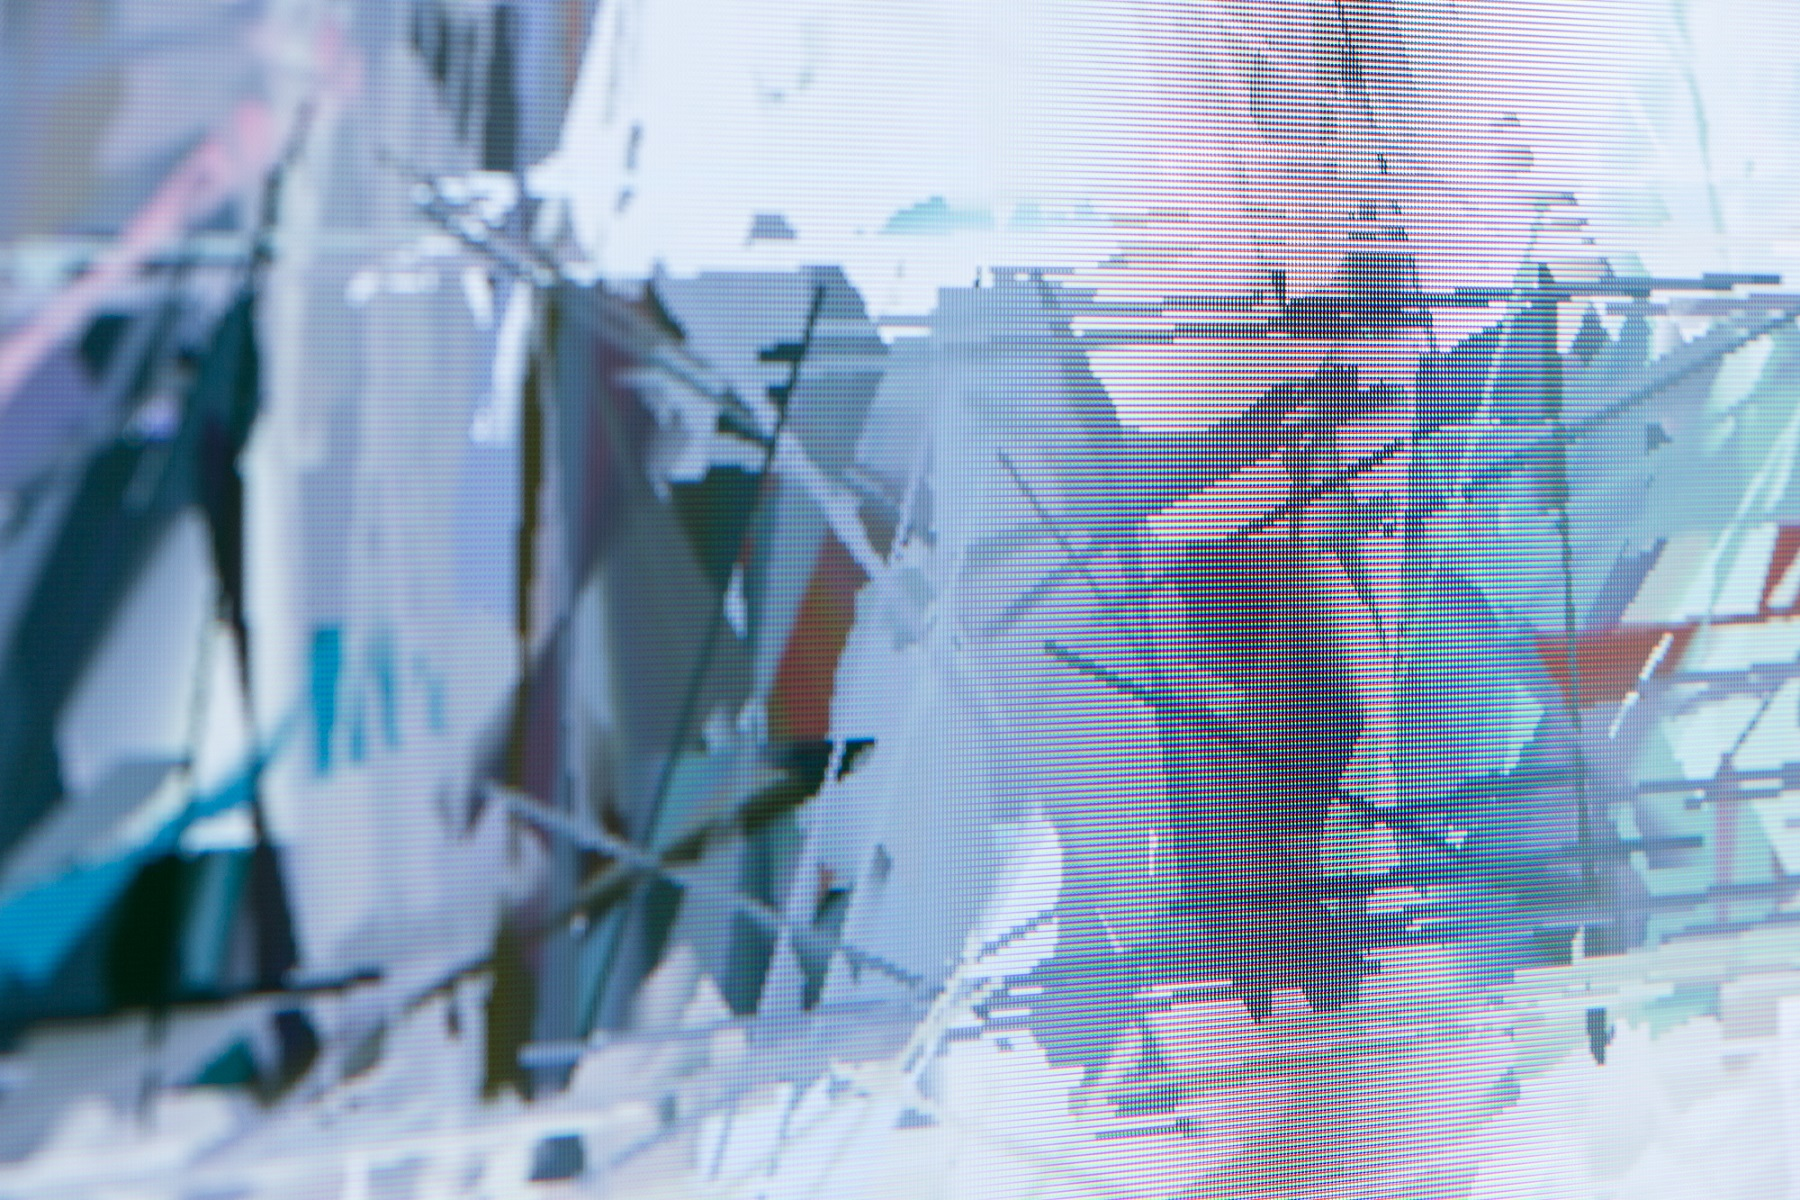
\includegraphics[width=0.8\textwidth]{img//mirror_example_1.jpg}
  \caption{丹尼爾.羅森的數位鏡面}\label{fig:mirror_example_1}
\end{figure}

在實作過程中,我發現許多參數會影響數位鏡面的效果,例如線條的長度與寬度等表層設定,或是每次刷新時繪製的線條數量等底層設定。此外,環境因素的變化也會影響數位鏡面的呈現效果。這些觀察激發了我的好奇心,使我想深入研究各種參數對數位鏡面效果的影響,進一步探索它背後的運作機制。

\subsection{二、研究目的}

\subsubsection{(一)了解不同參數設定對於數位鏡面的影響}
\subsubsection{(二)了解不同影像環境對於數位鏡面的影響}
\subsubsection{(三)探討不同環境與需求下數位鏡面的最優設定}

\newpage

\subsection{三、文獻探討}

\subsubsection{(一)數位鏡面}

數位鏡面最初是丹尼爾·羅森(2017)在機場捷運展示的一系列藝術作品。這些作品透過鏡頭捕捉現實世界的影像,並經由電腦計算處理後,以特殊的方式呈現在螢幕上。影像如圖\ref{fig:mirror_example_23}所示,經過數位化處理後,現實畫面顯得模糊且朦朧,營造出獨特的視覺效果。該系列中的每件作品皆展現了不同的風格與表現形式。本次實驗將聚焦於其中一種以類似線條形式呈現的數位鏡面作品,進行深入探討。

\begin{figure}[htbp]
  \centering
  % 第一張圖片
  \begin{minipage}[b]{0.45\textwidth}
    \centering
    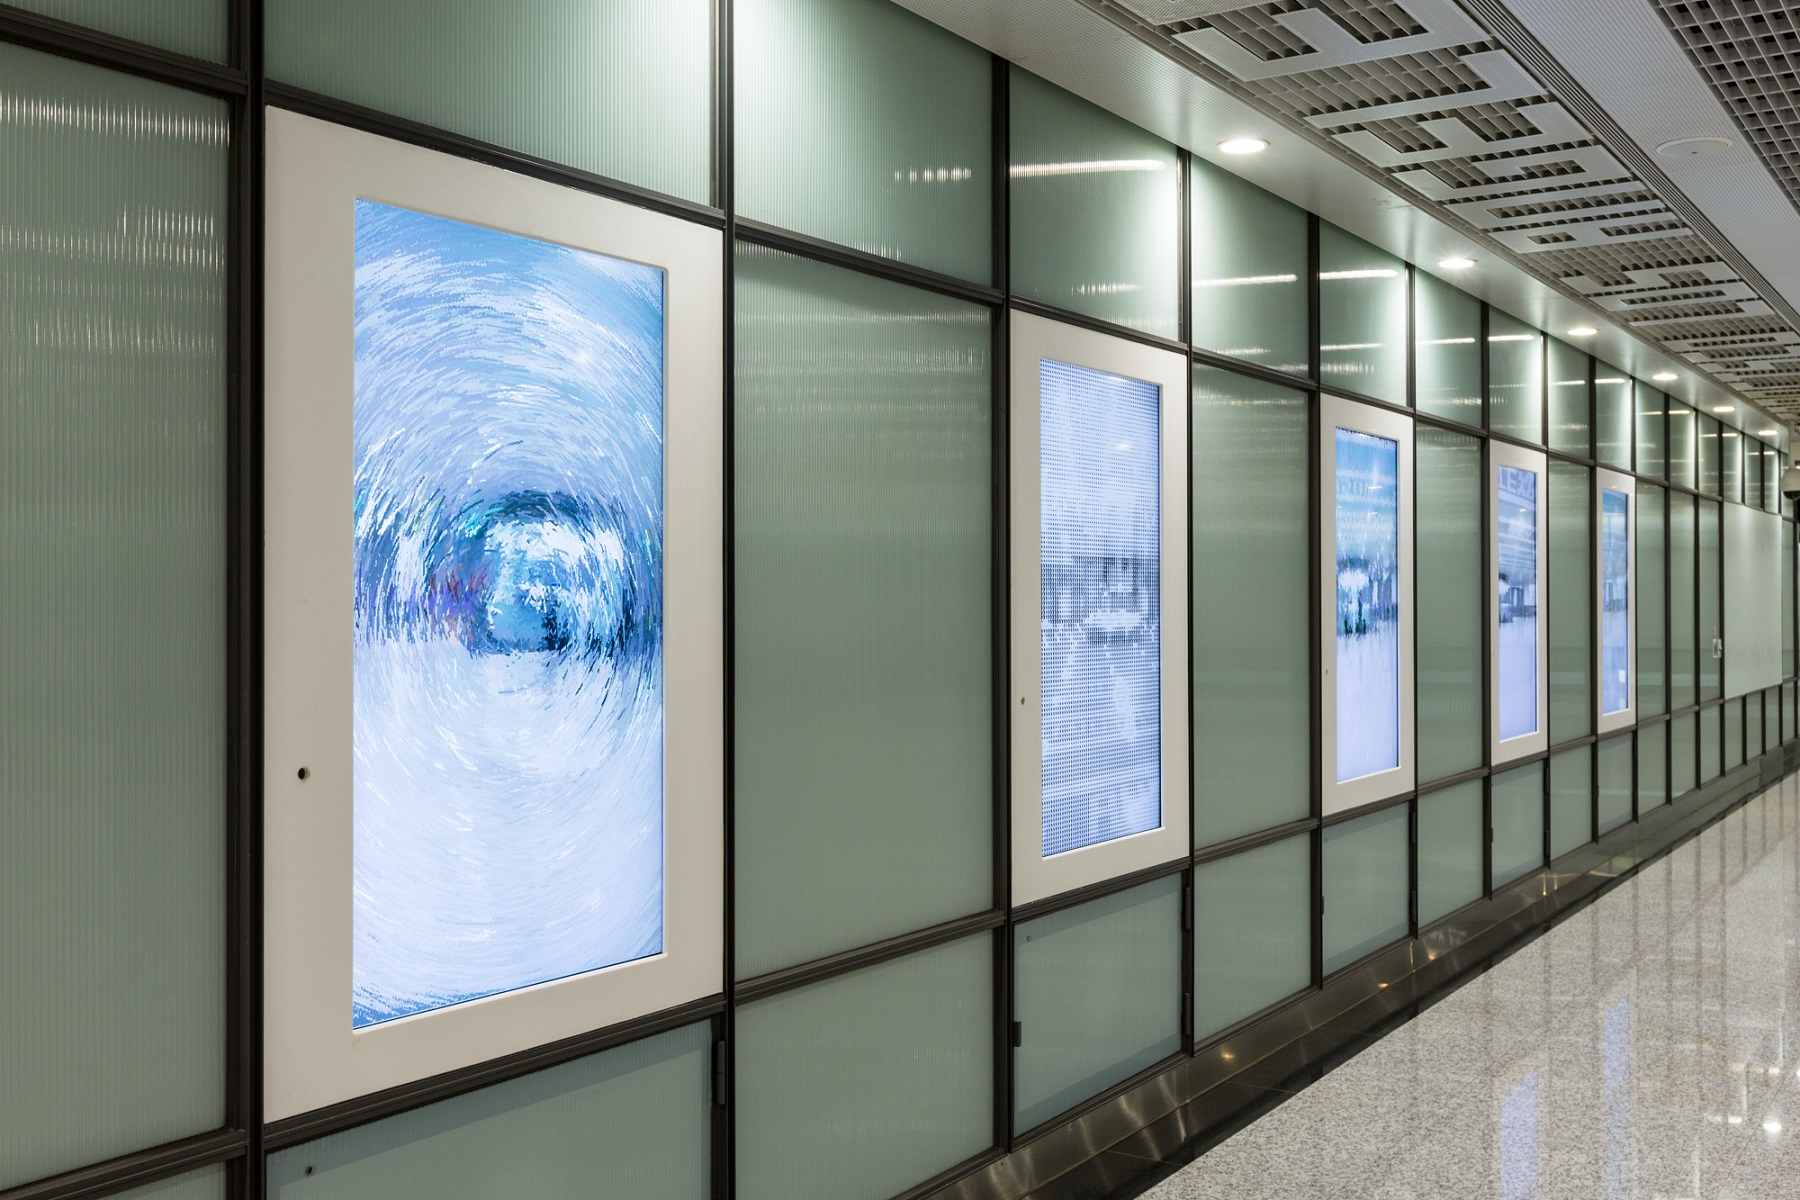
\includegraphics[width=\textwidth]{img/mirror_example_2.jpg}
  \end{minipage}
  \hfill
  % 第二張圖片
  \begin{minipage}[b]{0.45\textwidth}
    \centering
    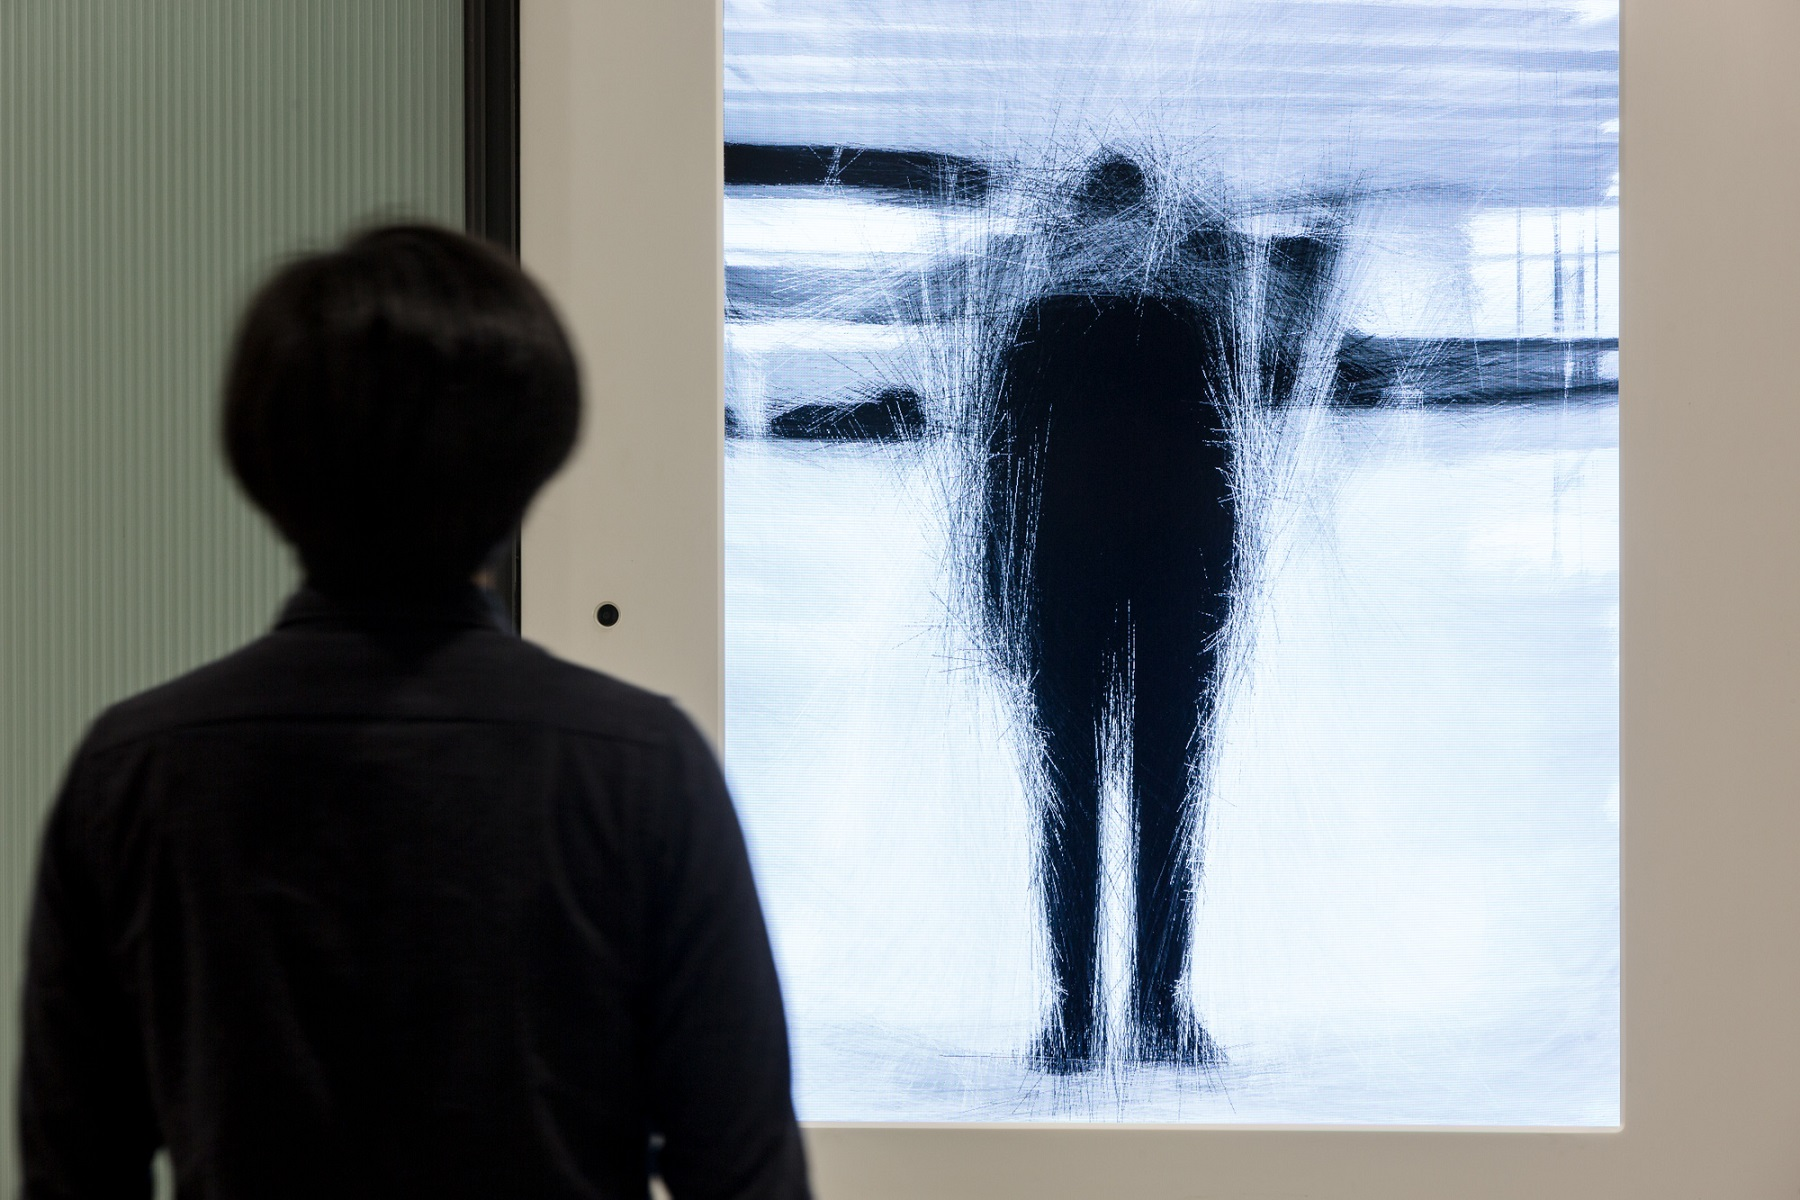
\includegraphics[width=\textwidth]{img/mirror_example_3.jpg}
  \end{minipage}
\caption{丹尼爾.羅森的數位鏡面}\label{fig:mirror_example_23}
\end{figure}

本次研究使用的是 happycorn 在 GitHub 上提供的數位鏡面模仿作品(2024)。程式中展示了以線條為主要呈現方式的數33位鏡面,其每一幀的繪製過程包括:讀取影像、繪製多條線條,以及刷新畫面。繪製線條的過程則可細分為以下步驟:模擬一條虛擬線、計算該線條路徑上所有像素點的平均值、以及根據計算結果繪製線條。更詳細的流程如圖\ref{fig:program_flaw}所示。

\begin{figure}[htbp]
  \centering
  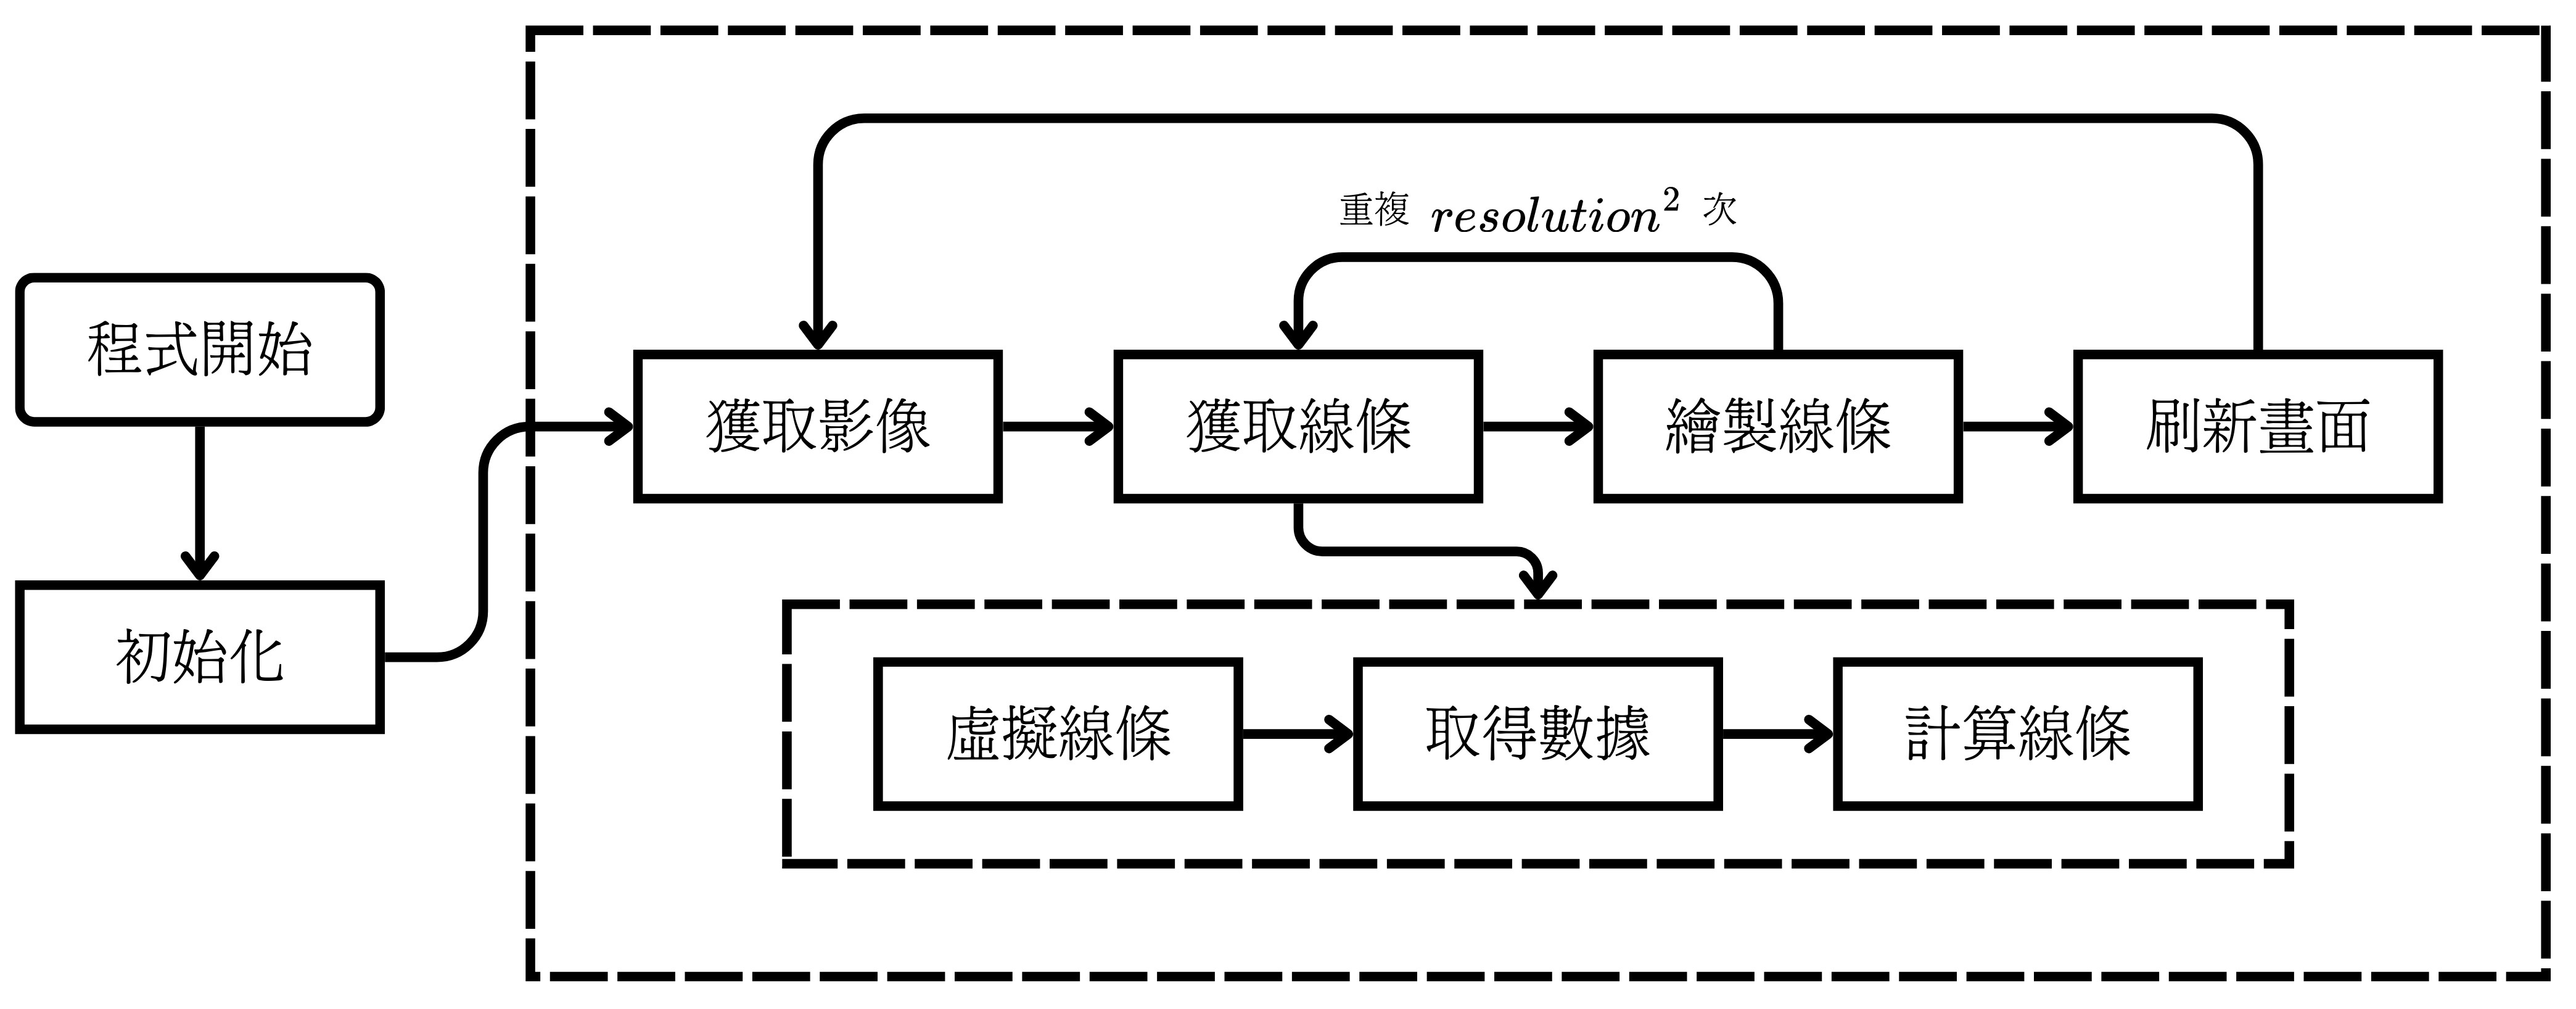
\includegraphics[width=0.8\textwidth]{img//program_flaw.jpg}
  \caption{數位鏡面流程圖}\label{fig:program_flaw}
\end{figure}

在整面數位鏡面中,可調整的參數有三項:線條寬度(width)、線條長度(length)與解析度(resolution)。線條寬度與長度分別表示數位鏡面在繪製時的線條寬度與長度;而解析度則是與繪製過程中的區域劃分相關。為了同時達成「繪製多條線」與「分散線條位置」的效果,作者透過 for 迴圈將整個鏡面切分為多個小方格,並在每個方格內繪製一條線,解析度即代表這些方格的寬度。

\subsubsection{(二)時間複雜度}

為了比較程式的計算速度,本研究引用了《Introduction to Algorithms》(Cormen et al., 2022)中關於執行時間(running time)的計算觀念。該觀念首先假設,在程式中第 $i$ 步的執行時間為常數 $c_i$。接著,針對輸入大小 $n$,寫出相應的操作步數。例如,若要透過 for 迴圈從長度為 $n$ 的陣列中找出最大值,則需要執行 $n \cdot c_i$ 次操作。

然而,直接這樣表示可能顯得過於繁瑣,因此可以進一步簡化為「增長的量級」。具體而言,只需保留最高次項,並忽略其係數,因為在輸入規模增長後,係數對總體增長的影響微乎其微。這樣的計算方式被翻譯成中文時,通常被稱為該演算法的「時間複雜度」。

\subsubsection{(三)Sum of absolute difference}

在本次實驗中,我需要計算圖片的相似度,為此將採用《Intelligent Image and Video Compression》(Bull \& Zhang, 2021)中提出的 Sum of Absolute Difference(SAD)演算法。該演算法針對兩張圖片 $s_1$ 和 $s_2$,計算它們之間的差異。

假設圖片 $s_1$ 和 $s_2$ 的尺寸為寬 $X$ 和高 $Y$,則 SAD 的計算方式如下:

\[
SAD = \sum_{x=0}^{X-1} \sum_{y=0}^{Y-1} \left| s_1[x, y] - s_2[x, y] \right|
\]

其中,$s_1[x, y]$ 和 $s_2[x, y]$ 分別表示兩張圖片在座標 $(x,y)$ 的像素值。若圖片為彩色,則需引入額外的色彩通道維度,分別計算每個通道的差異,並累加為最終結果。

\newpage

\section{貳、研究設備及器材}

\begin{table}[h]
  \centering
  \caption{研究設備與器材}
  \begin{tabular}{p{2cm}p{5cm}p{5cm}}
    \toprule
    類別 & 項目 & 型號或版本\\
    \midrule
    硬體 & 電腦乙台 & ASUS M3401QC\\
    軟體 & Python & 3.12.7 \\
        & Anaconda & 24.11.0 \\
        & Jupyter Notebook & 7.2.2 \\
        & OpenCV & 4.10.0 \\
        & NumPy & 2.1.3 \\
        & Matplotlib & 3.9.2 \\
    \bottomrule
  \end{tabular}
\end{table}

\newpage

\section{參、研究過程與方法}

\subsection{一、研究架構圖}

\begin{figure}[htbp]
  \centering
  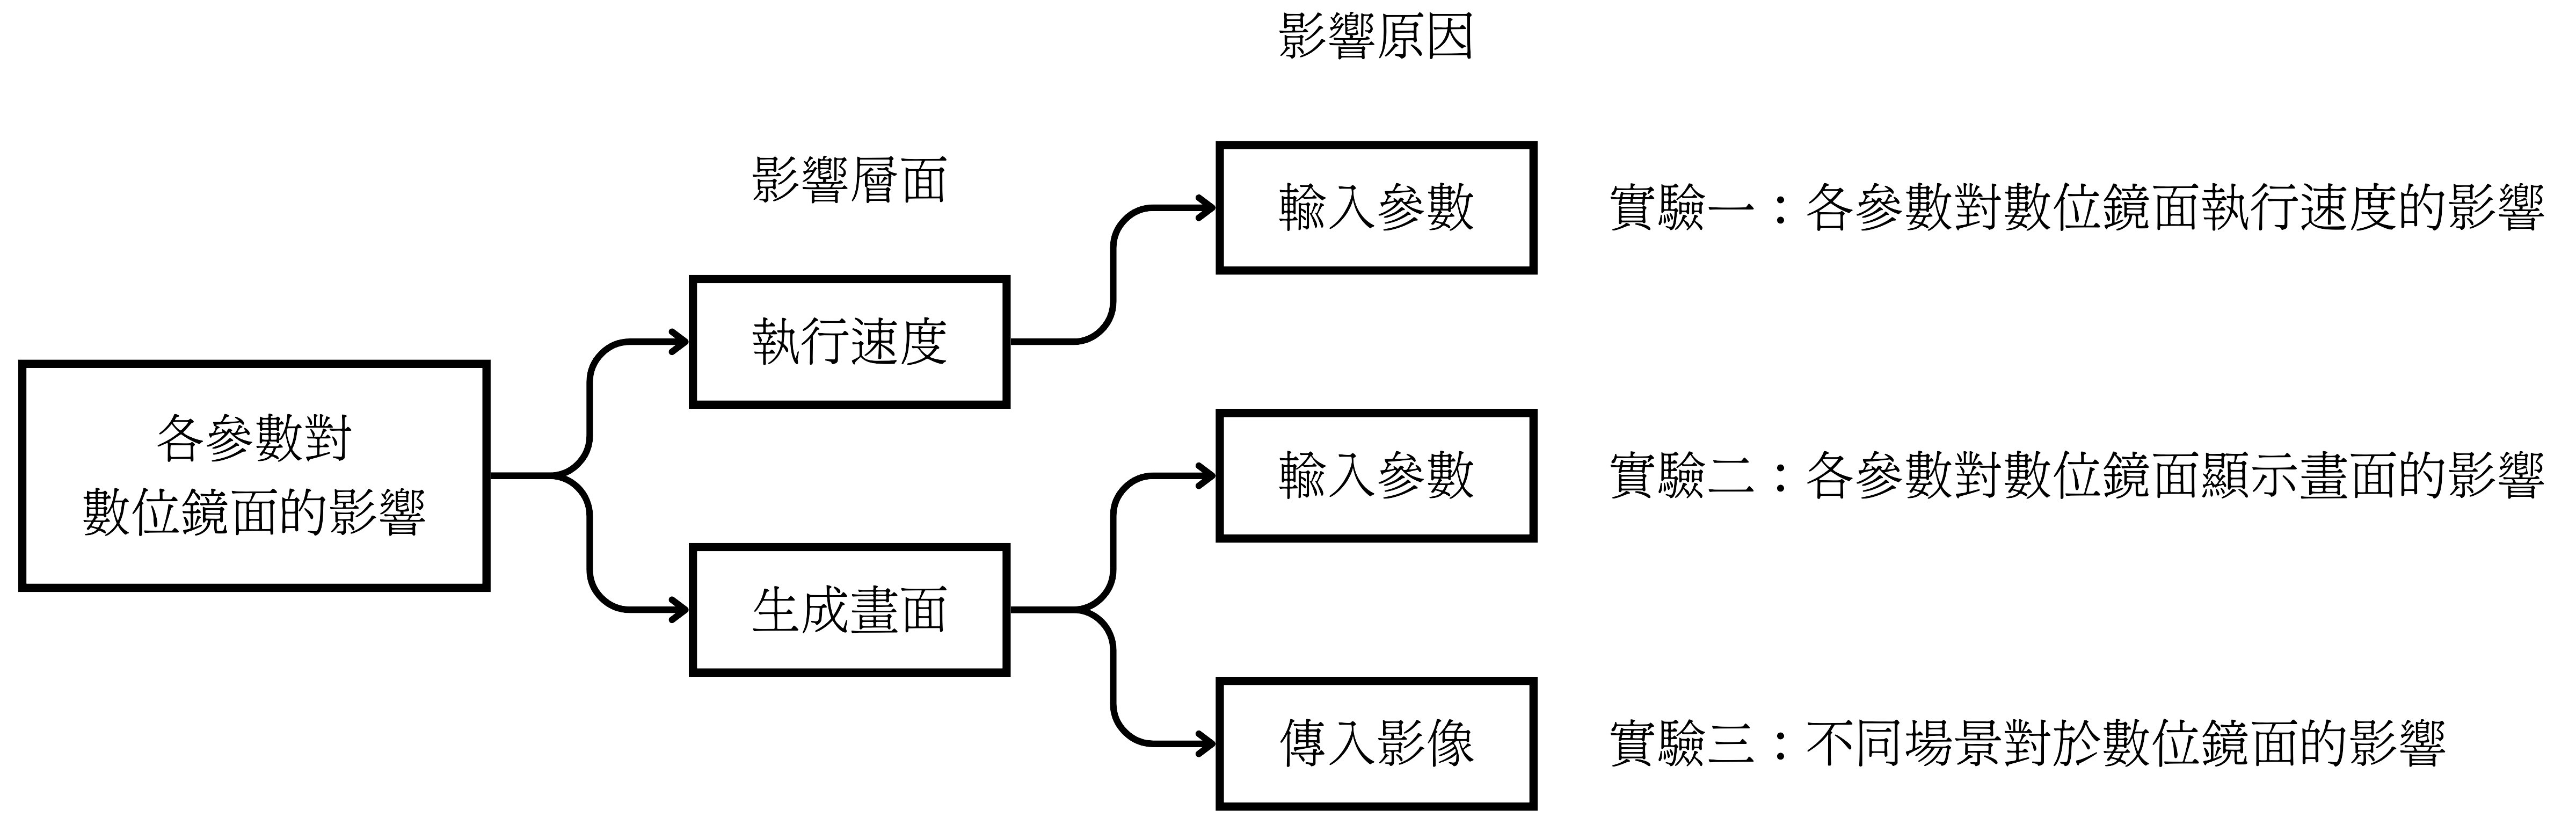
\includegraphics[width=0.8\textwidth]{img//research_flaw.png}
  \caption{研究架構圖}
\end{figure}

\subsection{二、實驗一:各參數對數位鏡面執行速度的影響}

為了分析數位鏡面程式的執行速度及其影響因素,本實驗記錄程式的執行時間,並探討可調整參數(線條寬度、線條長度及解析度)對每幀渲染時間與單條線條繪製時間的影響。實驗設計如表\ref{table:sc1_des} 所示。

\begin{table}[h]
  \centering
  \caption{執行速度與參數關係的實驗設計}\label{table:sc1_des}
  \begin{tabular}{p{0.2cm}p{3.5cm}p{4.5cm}p{6cm}}
    \toprule
      & 操縱變因 & 應變變因 & 控制變因 \\ 
    \midrule
    1 & 線條寬度(width) & 繪製一條線所需的時間 & 線條長度、解析度等其他參數 \\ 
    2 & 線條長度(length) & 繪製一條線所需的時間 & 線條寬度、解析度等其他參數 \\ 
    3 & 線條寬度(width) & 繪製每幀所需的時間 & 線條長度、解析度等其他參數 \\ 
    4 & 線條長度(length) & 繪製每幀所需的時間 & 線條寬度、解析度等其他參數 \\ 
    5 & 解析度(resolution) & 繪製每幀所需的時間 & 線條寬度、線條長度等其他參數 \\ 
    \bottomrule
  \end{tabular}
\end{table}

在實驗設計中,每組實驗將重複執行 100 次,並計算所得結果的平均值以作為最終數據。非操縱變因的參數均固定為預設初始值,其中線條寬度(width)設定為 5,線條長度(length)設定為 100,解析度(resolution)設定為 100。

\subsection{三、實驗二:各參數對數位鏡面顯示畫面的影響}

數位鏡面在繪製過程中,當畫面發生變化時,所呈現的內容會逐漸接近現實場景,直至達到一定相似程度後停止變化。這一階段被稱為穩定狀態。本實驗主要觀察兩項指標:一是數位鏡面進入穩定狀態後與現實的差異,二是畫面變動後達到穩定狀態所需的時間。

在實驗中,我將數值分別設定為以下範圍:線條寬度(width)為 1 至 41,間隔 2;線條長度(length)為 1 至 501,間隔 25;解析度(resolution)為 10 至 510,間隔 25。值得說明的是,解析度的起始值設定為 10,這是基於實驗一的結果推算得知,若將解析度設為 1,運算時間將增加至預設值的 $10^4$ 倍,不僅超出實際應用的可能性,也難以有效控制實驗時間。因此,解析度選擇從 10 開始,該設定的運算時間約為預設值的 $10^2$ 倍,既符合實驗條件要求,也更接近實際應用場景。

為了量化數位鏡面與現實場景之間的相似程度,本研究採用前述文獻探討中提及的 SAD 演算法。為使計算結果更具直觀性,將 SAD 值歸一化為百分比形式,其方法為將 SAD 值除以理論最大值,公式如下。其中,$X$ 和 $Y$ 分別表示圖片的寬度與高度,$255$ 為像素值的最大可能差異。

\[
SAD_{\text{normalized}} = \frac{\sum_{x=0}^{X-1} \sum_{y=0}^{Y-1} \left| s_1[x, y] - s_2[x, y] \right|}{X \cdot Y \cdot 255}
\]

SAD 結果的形態預期與分布如圖\ref{fig:test_img2} 所示。為判定穩定狀態,數據被劃分為 20 組,並將出現頻率最高的組別作為穩定狀態的指標。當實驗數據逐漸收斂至該組別,即可判定實驗已達穩定狀態。

\begin{figure}[htbp]
  \centering
  \begin{minipage}[b]{0.45\textwidth}
    \centering
    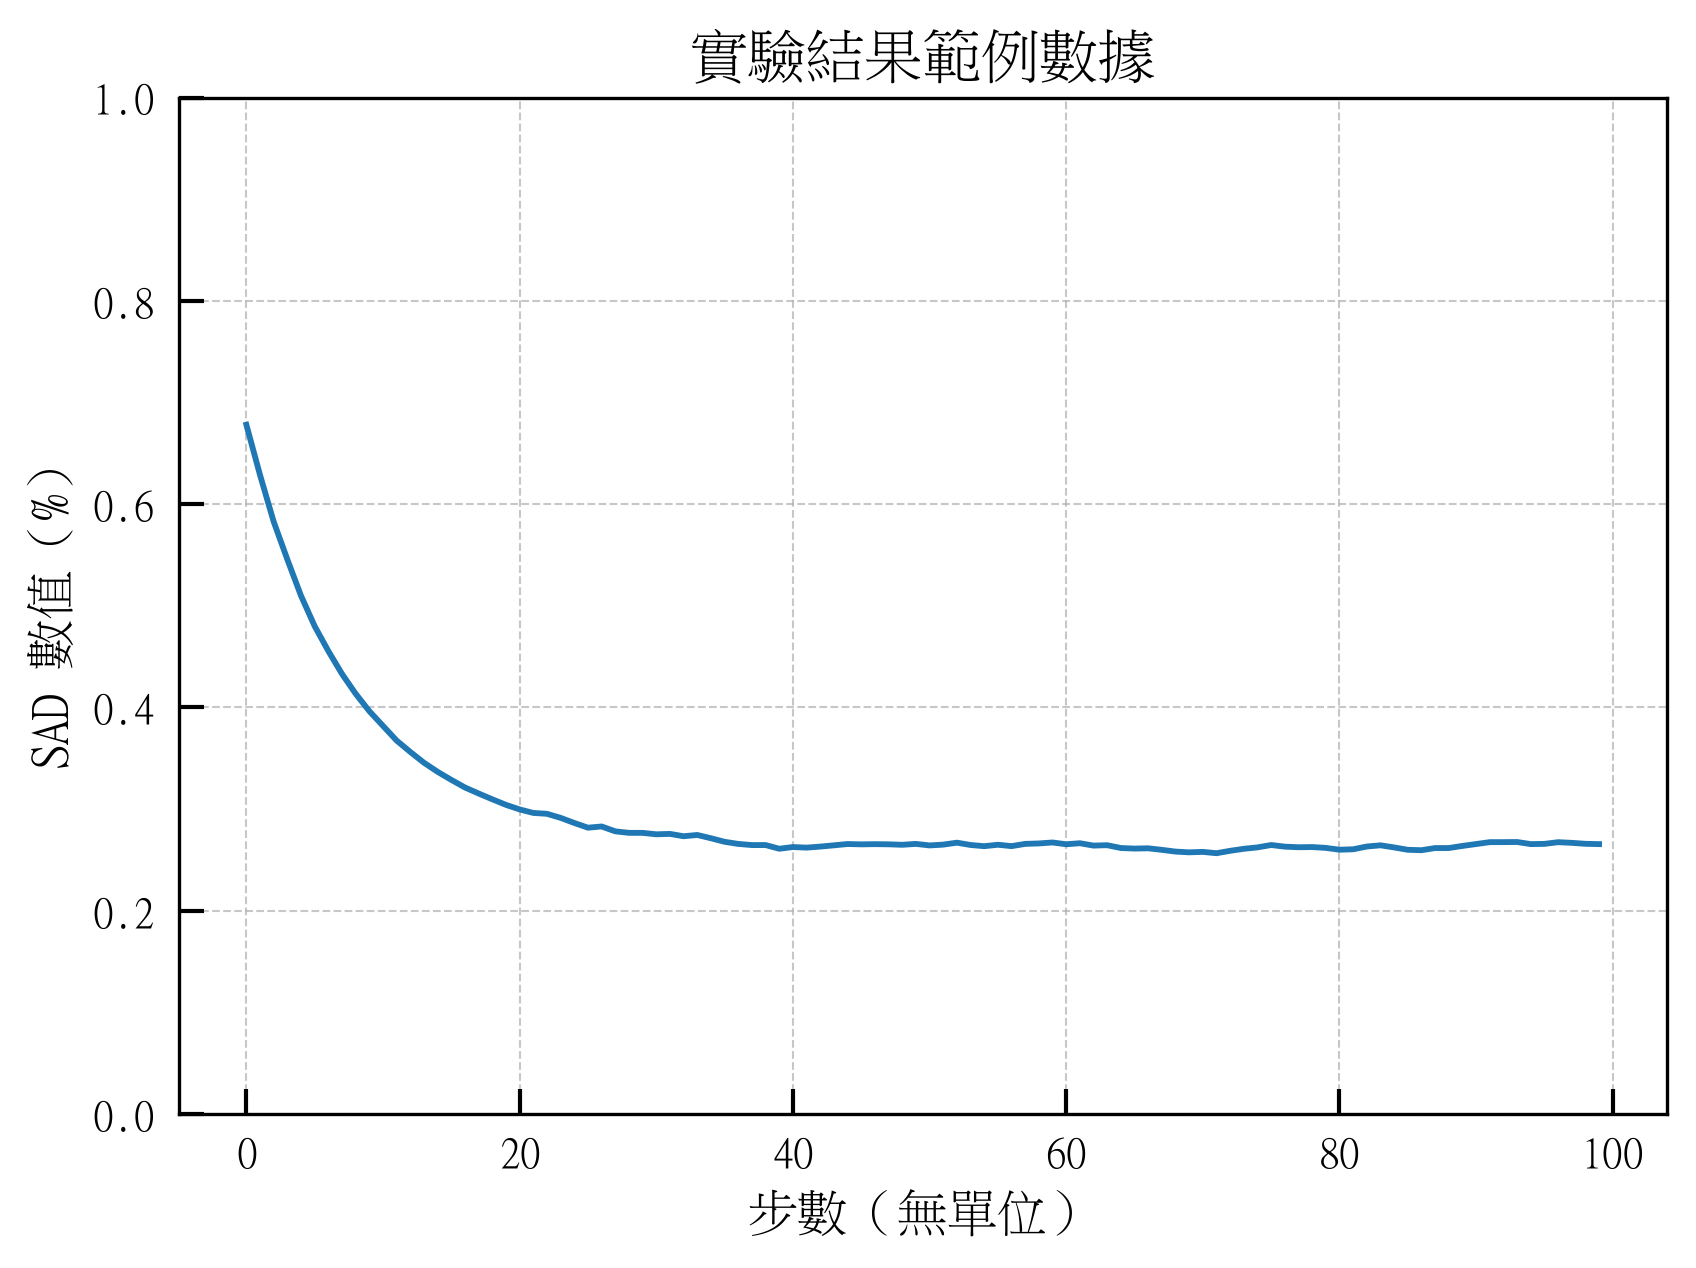
\includegraphics[width=\textwidth]{img/SAD_expriment_example_1.png}
  \end{minipage}
  \hfill
  \begin{minipage}[b]{0.45\textwidth}
    \centering
    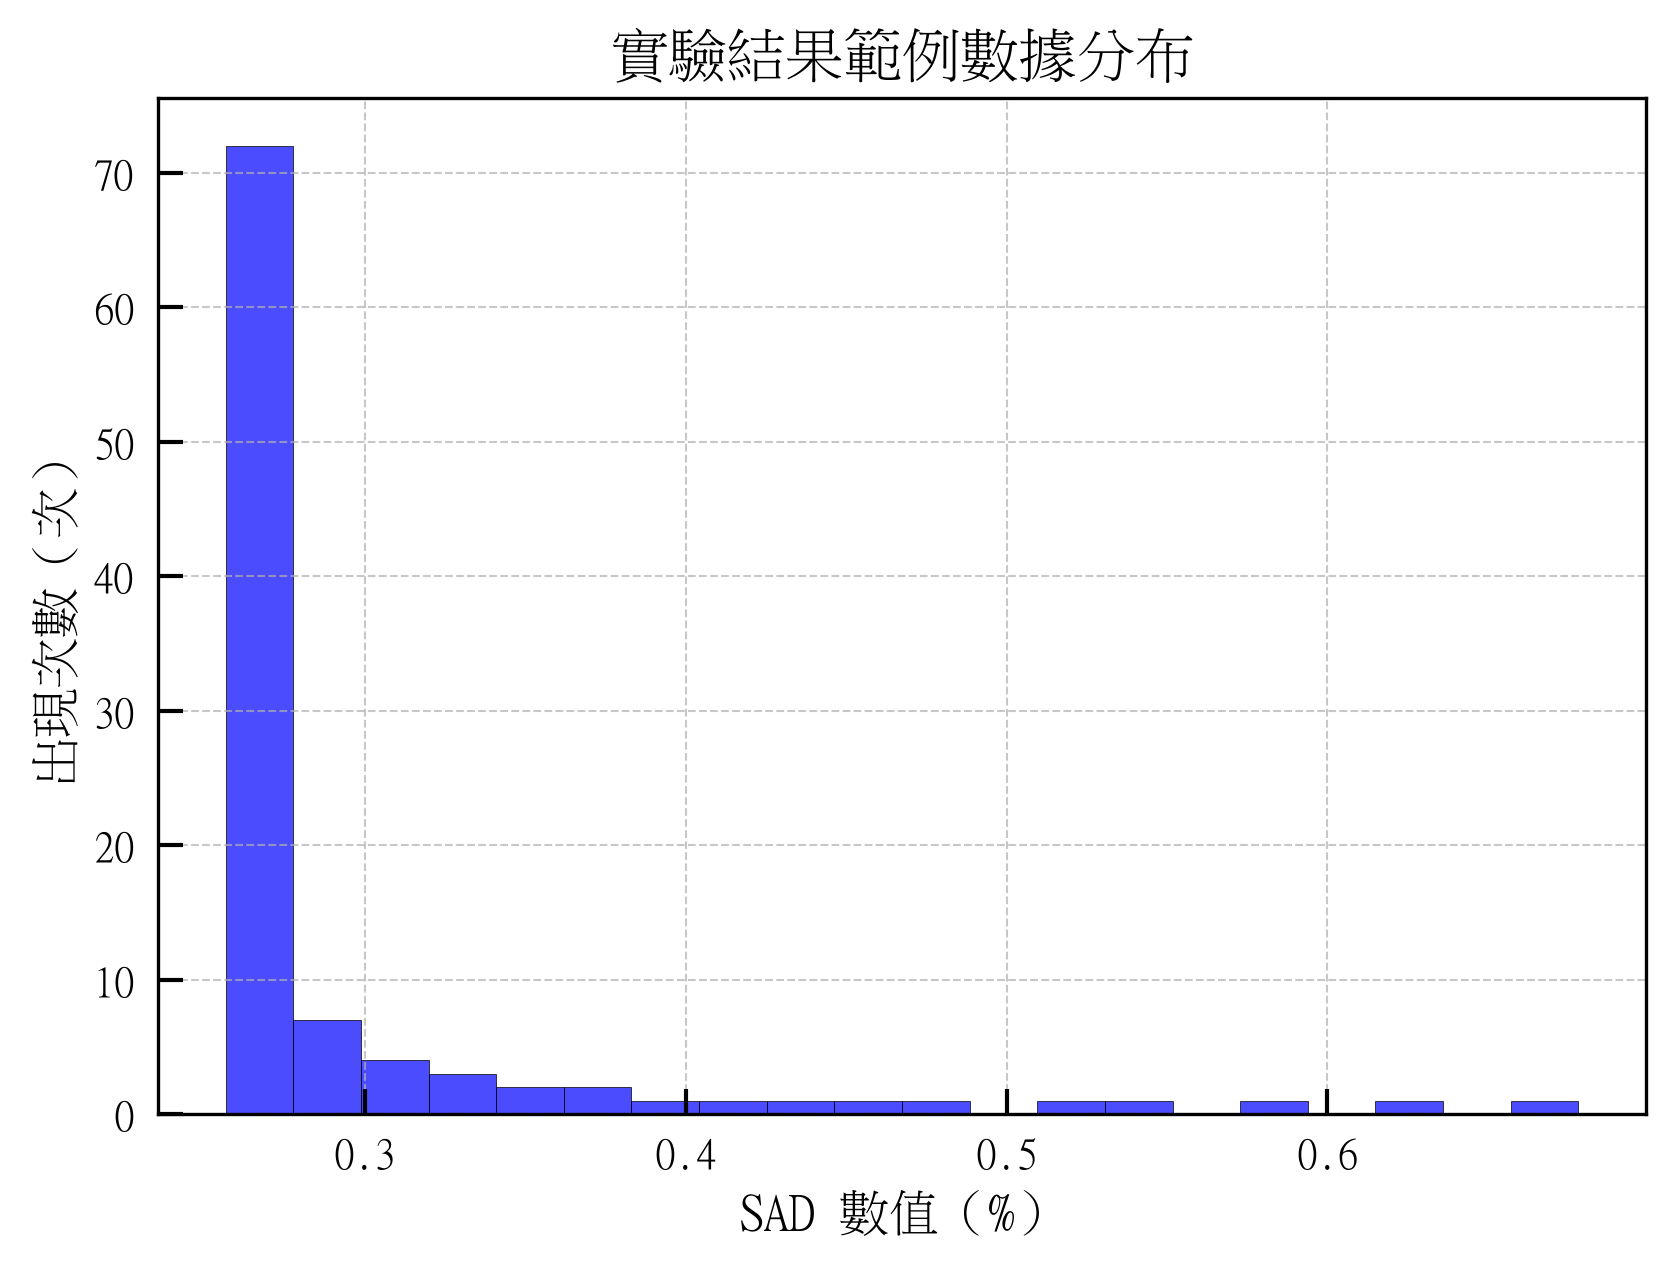
\includegraphics[width=\textwidth]{img/SAD_expriment_example_2.png}
  \end{minipage}
  \caption{實驗結果範例數據}\label{fig:test_img2}

\end{figure}

此外,為了統一不同參數下的測試條件,我選用了三組特定的測試圖片,分別為白藍交錯、紅黑交錯與紅黃交錯的圖案,作為數位鏡面的輸入來源。具體圖片如圖\ref{fig:test_img1} 所示。

\begin{figure}[htbp]
  \centering
  \begin{minipage}[b]{0.3\textwidth}
    \centering
    
\includegraphics[width=\textwidth]{img/blank_blue.png}
  \end{minipage}
  \hfill
  \begin{minipage}[b]{0.3\textwidth}
    \centering
    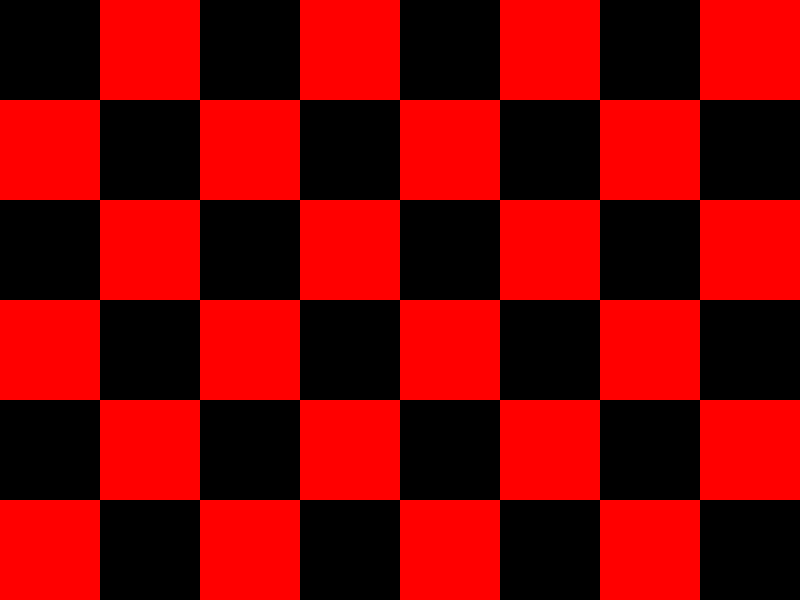
\includegraphics[width=\textwidth]{img/blank_red.png}
  \end{minipage}
  \hfill
  \begin{minipage}[b]{0.3\textwidth}
    \centering
    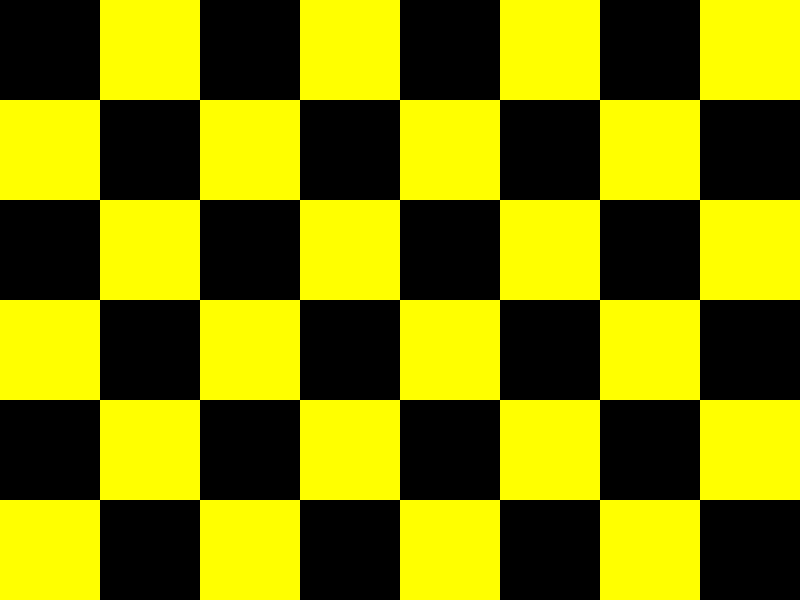
\includegraphics[width=\textwidth]{img/blank_Yellow.png}
  \end{minipage}
  \caption{測試照片}\label{fig:test_img1}
\end{figure}

\newpage

\subsection{四、實驗三:不同場景對於數位鏡面的影響}

為探討不同場景對於數位鏡面的影響,我將場景可能不同的點列為:總體場景的複雜程度、總體場景的顏色數量與總體的顏色差異程度。

為了模擬這三種不同的向度,我將製作幾種圖片分別對應他們。總體場景的複雜程度我透過將畫面切分成 12 塊、48 塊、192 塊的方式模擬。總體場景的顏色數量我將其分成 2 種、3 種(紅、綠、藍)與 6 種(紅、綠、藍、黃、青、紫)顏色。

總體的顏色差異程度因為在顏色多的狀況下難以量化,因此只對 2 種顏色的組別做測試,顏色分別是黑搭配紅、綠、藍、黃、青、紫與白七色。

實驗設計表如下:

\begin{table}[h]
  \centering
  \caption{不同場景複雜程度與顏色數量影響的實驗設計}\label{table:sc3_des}
  \begin{tabular}{p{1cm}p{3cm}p{3cm}p{3cm}}
    \toprule
    & 12 塊 & 48 塊 & 192 塊 \\ 
    \midrule
    三種 & 紅、綠、藍 & 紅、綠、藍 & 紅、綠、藍 \\ 
    六種 & 紅、綠、藍、 & 紅、綠、藍、 & 紅、綠、藍、 \\ 
    & 黃、橘、紫 & 黃、橘、紫 & 黃、橘、紫 \\ 
    \bottomrule
  \end{tabular}
  \begin{tabular}{p{1cm}p{3cm}p{3cm}p{3cm}}
    \toprule
    & 12 塊 & 48 塊 & 192 塊 \\ 
    \midrule
    兩種 & 紅 & 紅 & 紅 \\ 
    & 綠 & 綠 & 綠 \\ 
    & 藍 & 藍 & 藍 \\ 
    & 黃 & 黃 & 黃 \\ 
    & 青 & 青 & 青 \\ 
    & 紫 & 紫 & 紫 \\ 
    & 白 & 白 & 白 \\ 
    \bottomrule
  \end{tabular}
\end{table}

\newpage

\section{肆、研究結果}

\subsection{一、實驗一:各參數對數位鏡面執行速度的影響}

實驗結果如圖\ref{fig:result_1}。在圖 a, b 中可以看到,線條寬度無論對應哪個組別都與執行時間呈現低度相關。而在圖 c, d 的線條長度雖然在單條現實呈現低度相關,但當到繪製單幀時,其呈現出高度相關。最後,圖 e 的解析度與執行時間呈現負指數相關。

\begin{figure}[htbp]
  \centering
  % 第一行圖片
  \begin{subfigure}{0.45\textwidth}
      \centering
      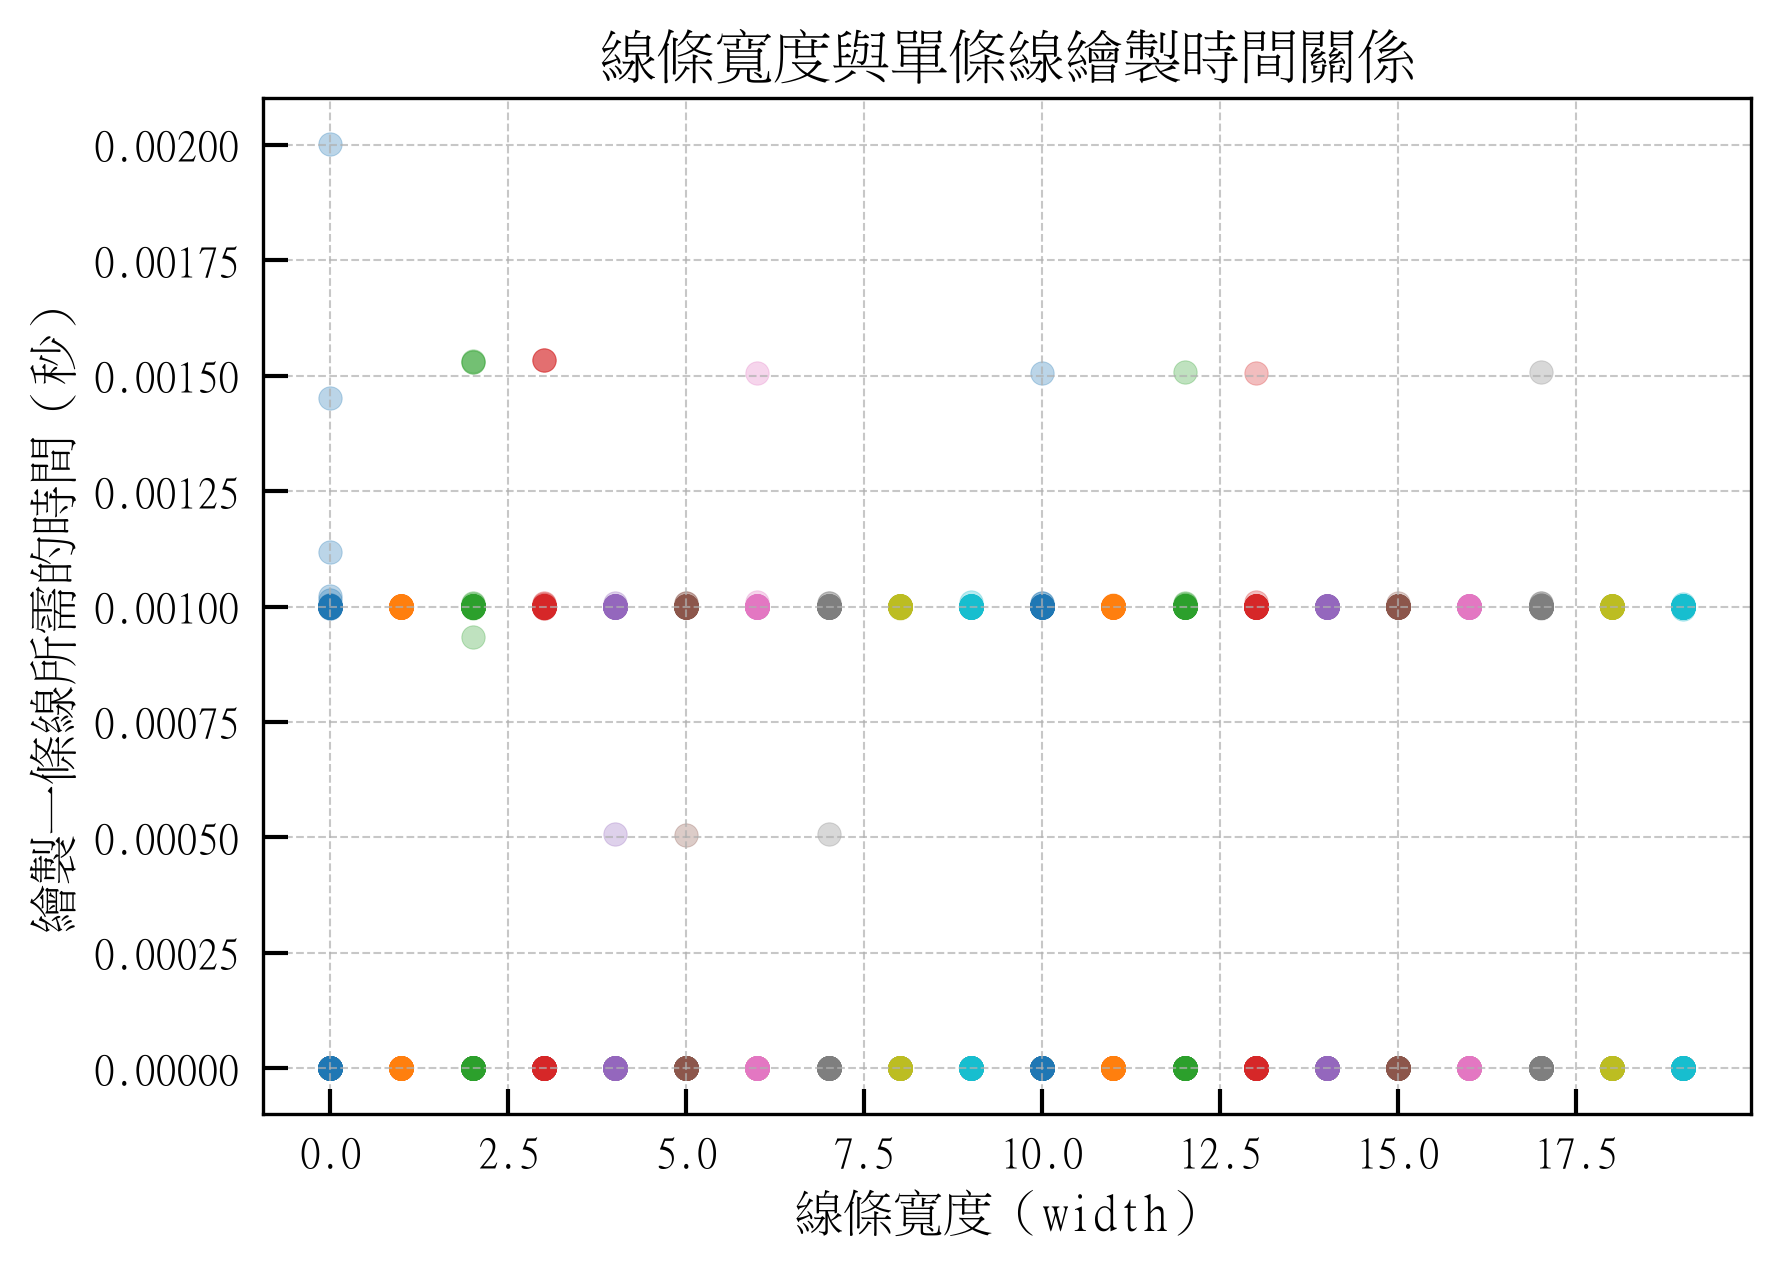
\includegraphics[width=\linewidth]{img/OutputImg/_Time_l-w.png} % 替換為你的圖片路徑
      \caption{線條寬度與單條線繪製時間關係}
  \end{subfigure}
  \begin{subfigure}{0.45\textwidth}
      \centering
      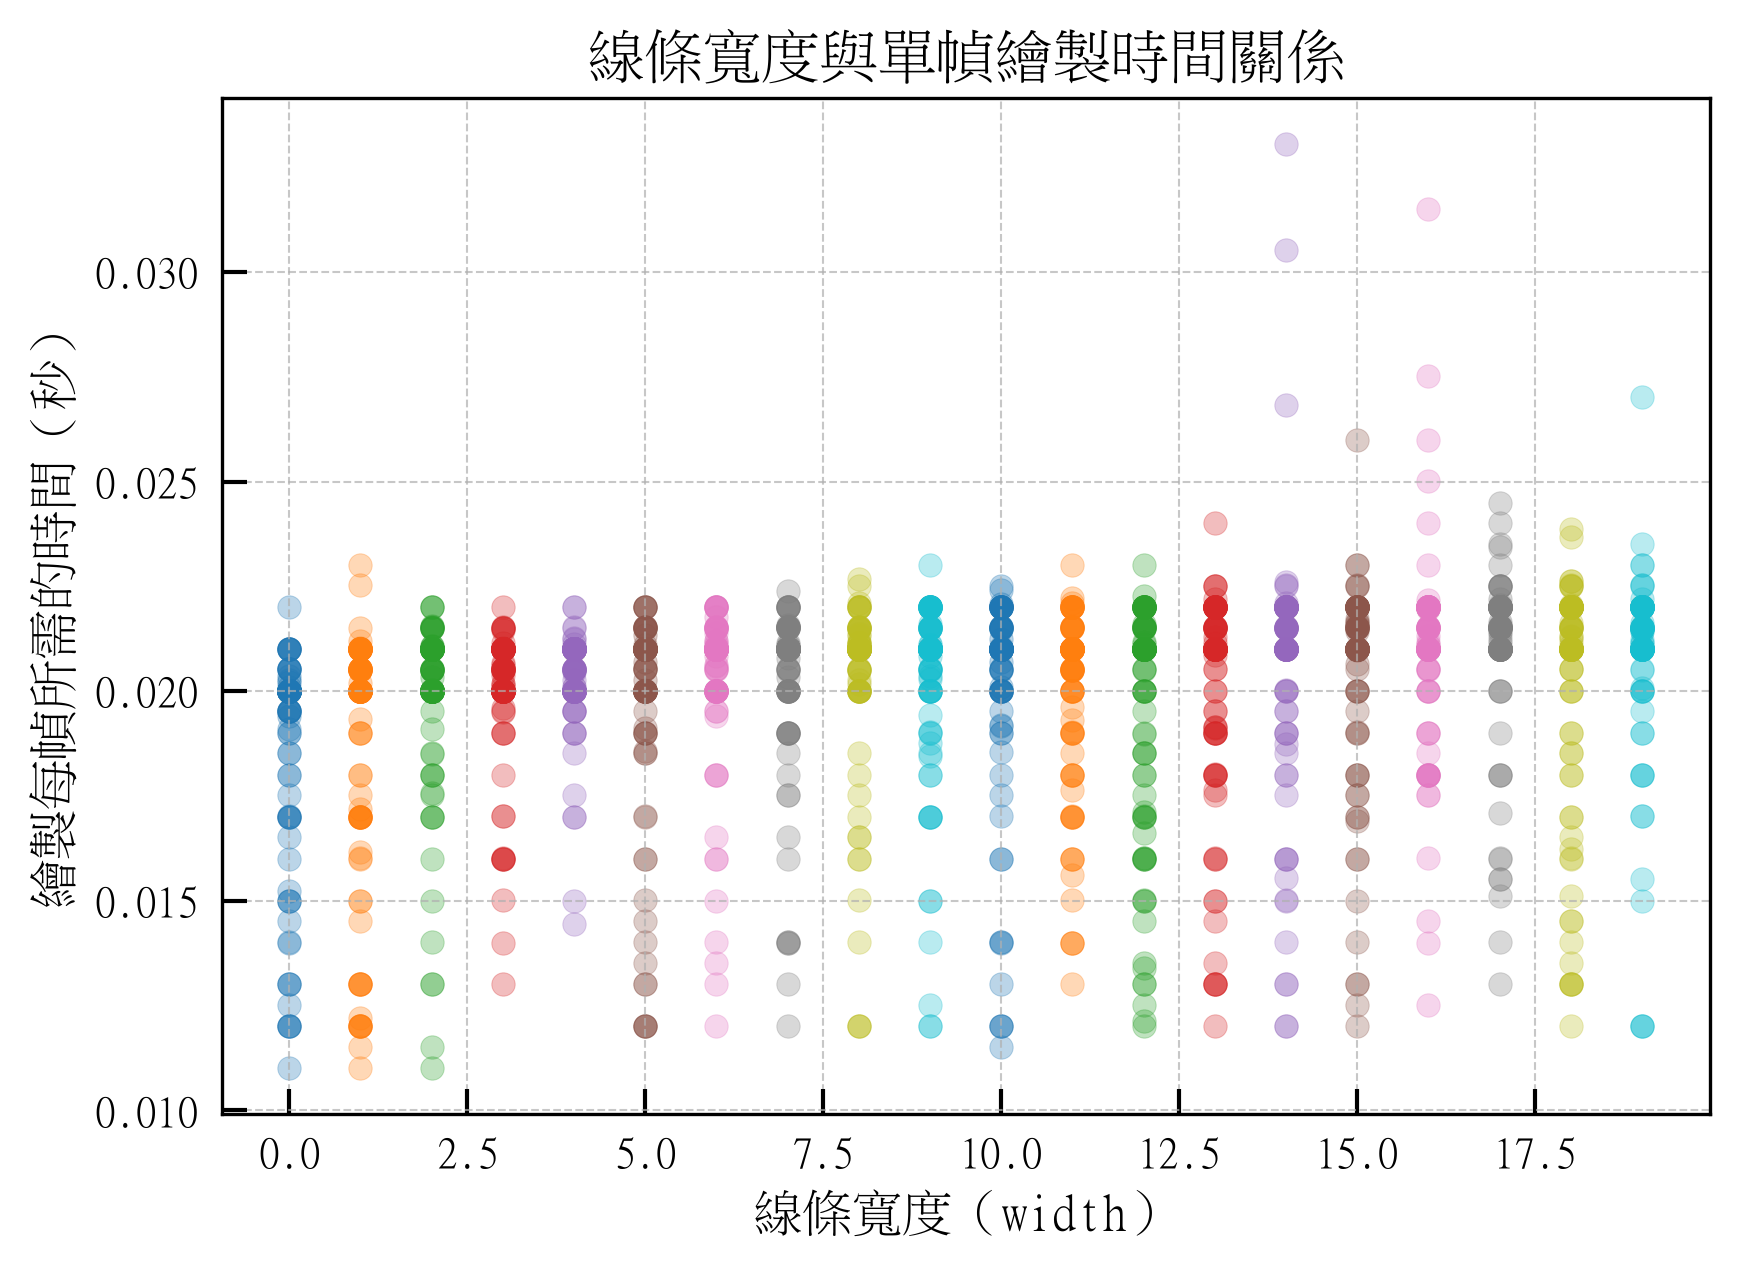
\includegraphics[width=\linewidth]{img/OutputImg/_Time_f-w.png} % 替換為你的圖片路徑
      \caption{線條寬度與單幀繪製時間關係}
  \end{subfigure}
  
  % 第二行圖片
  \begin{subfigure}{0.45\textwidth}
      \centering
      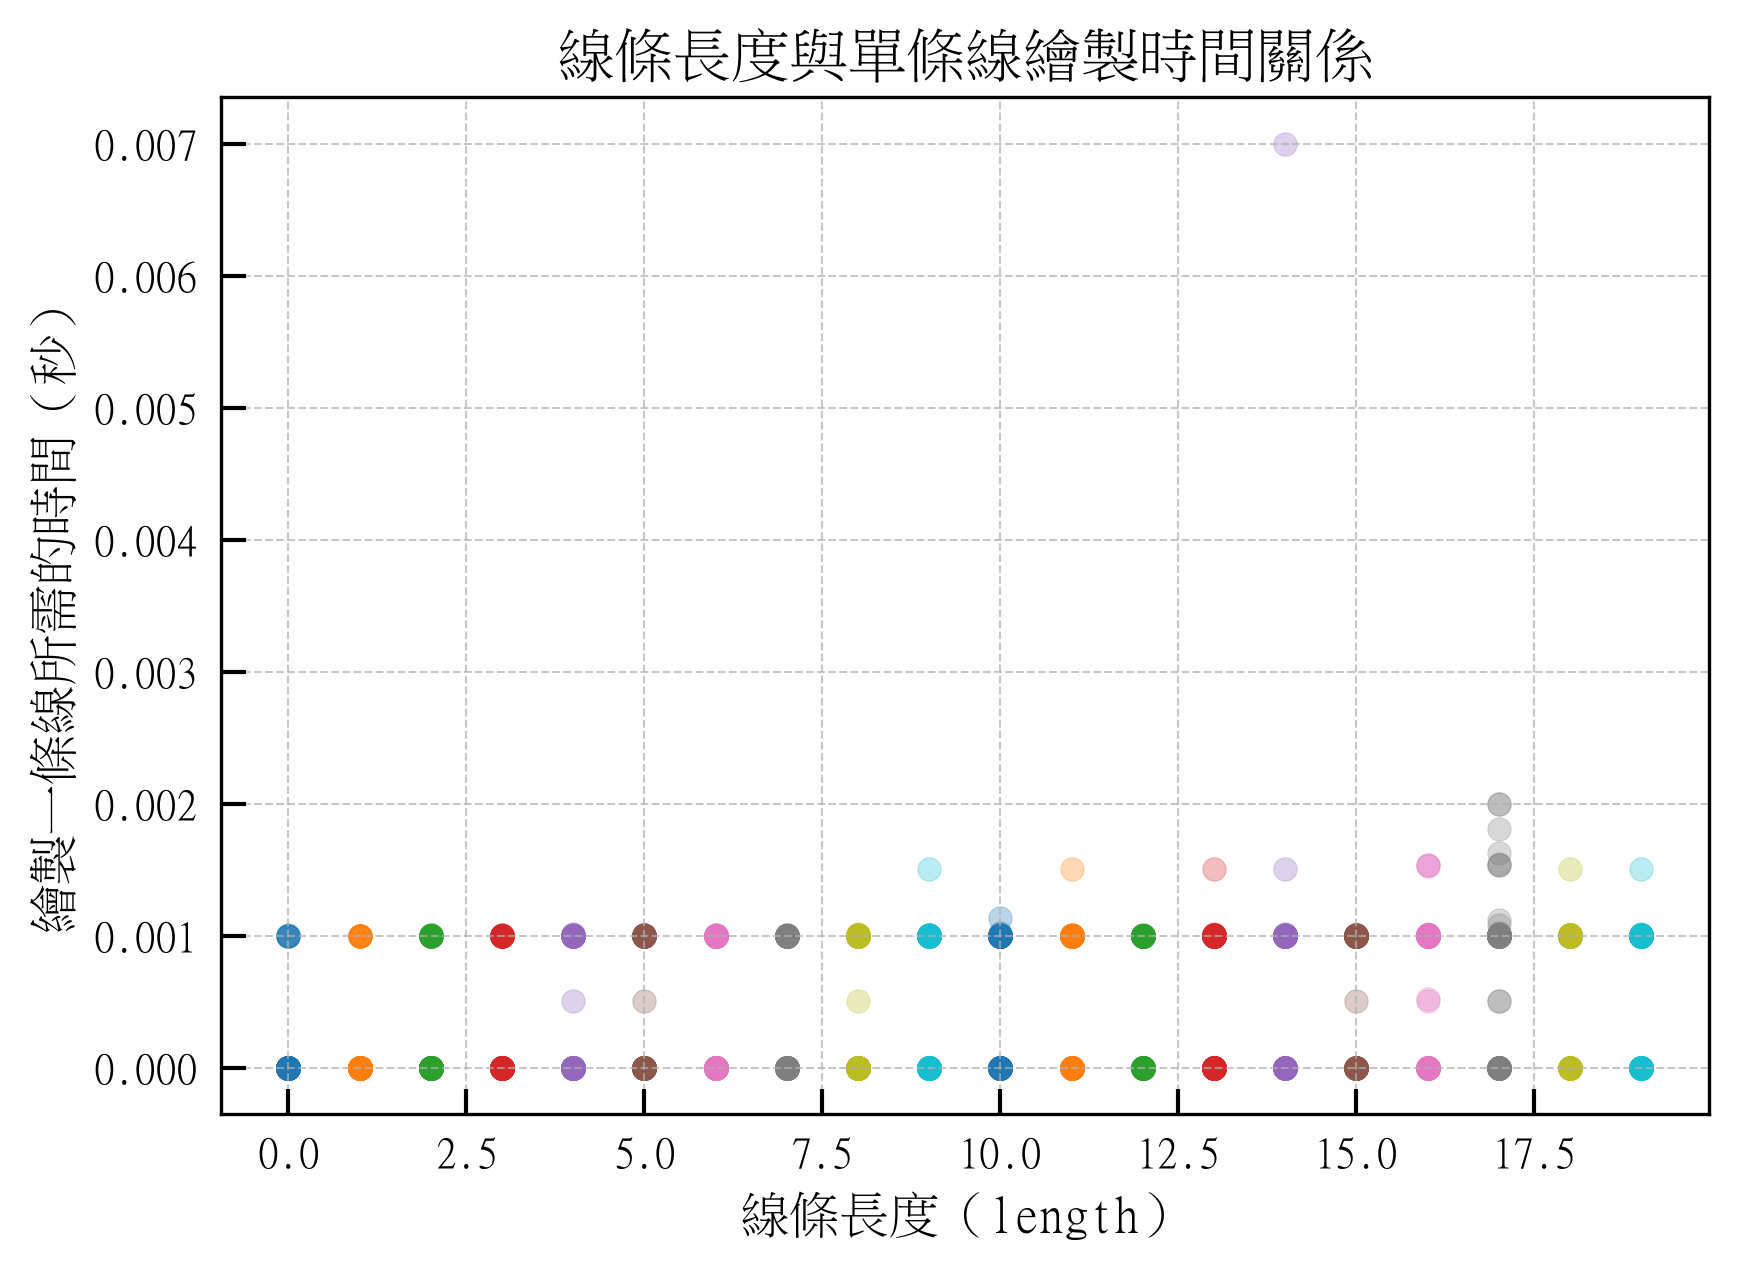
\includegraphics[width=\linewidth]{img/OutputImg/_Time_l-l.png} % 替換為你的圖片路徑
      \caption{線條長度與單條線繪製時間關係}
  \end{subfigure}
  \begin{subfigure}{0.45\textwidth}
      \centering
      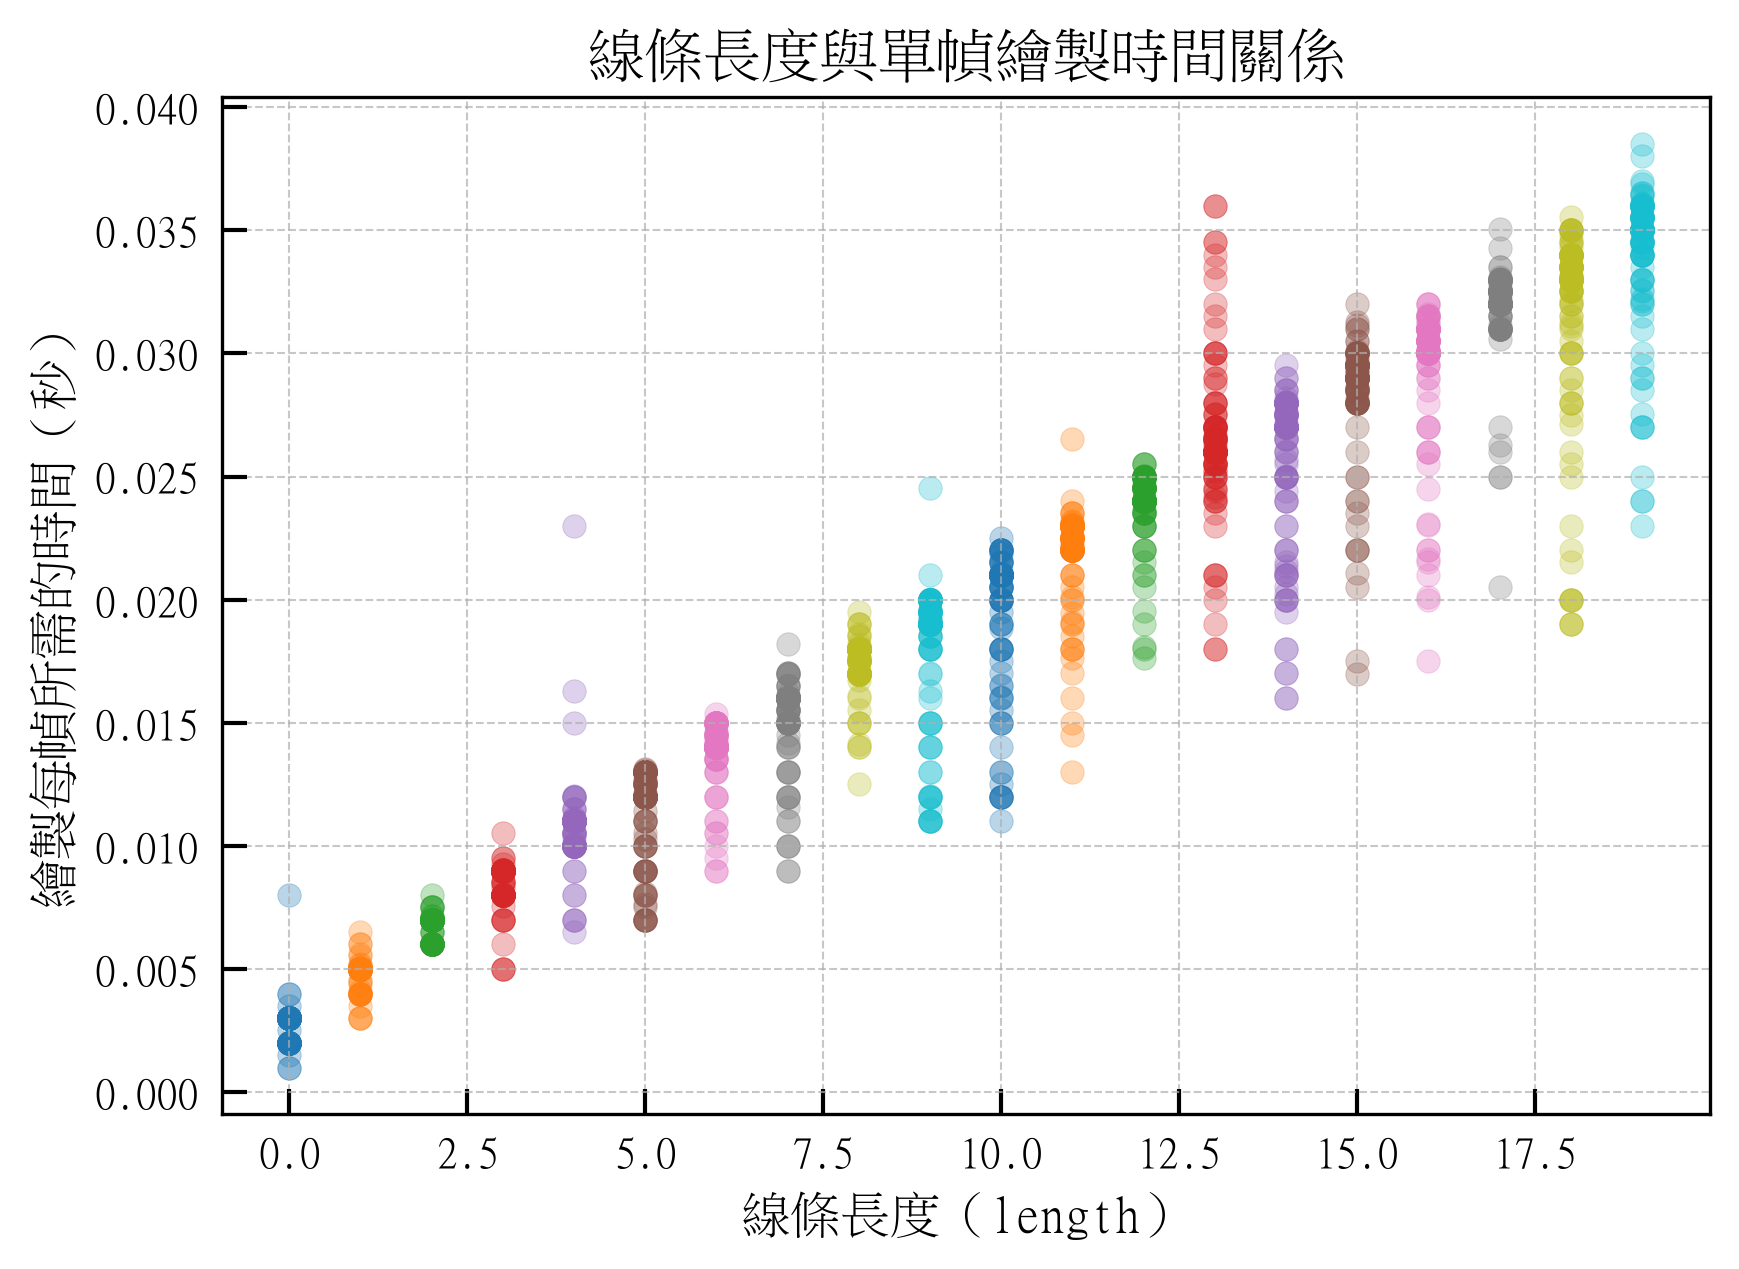
\includegraphics[width=\linewidth]{img/OutputImg/_Time_f-l.png} % 替換為你的圖片路徑
      \caption{線條長度與單幀繪製時間關係}
  \end{subfigure}

  \begin{subfigure}{0.45\textwidth}
      \centering
      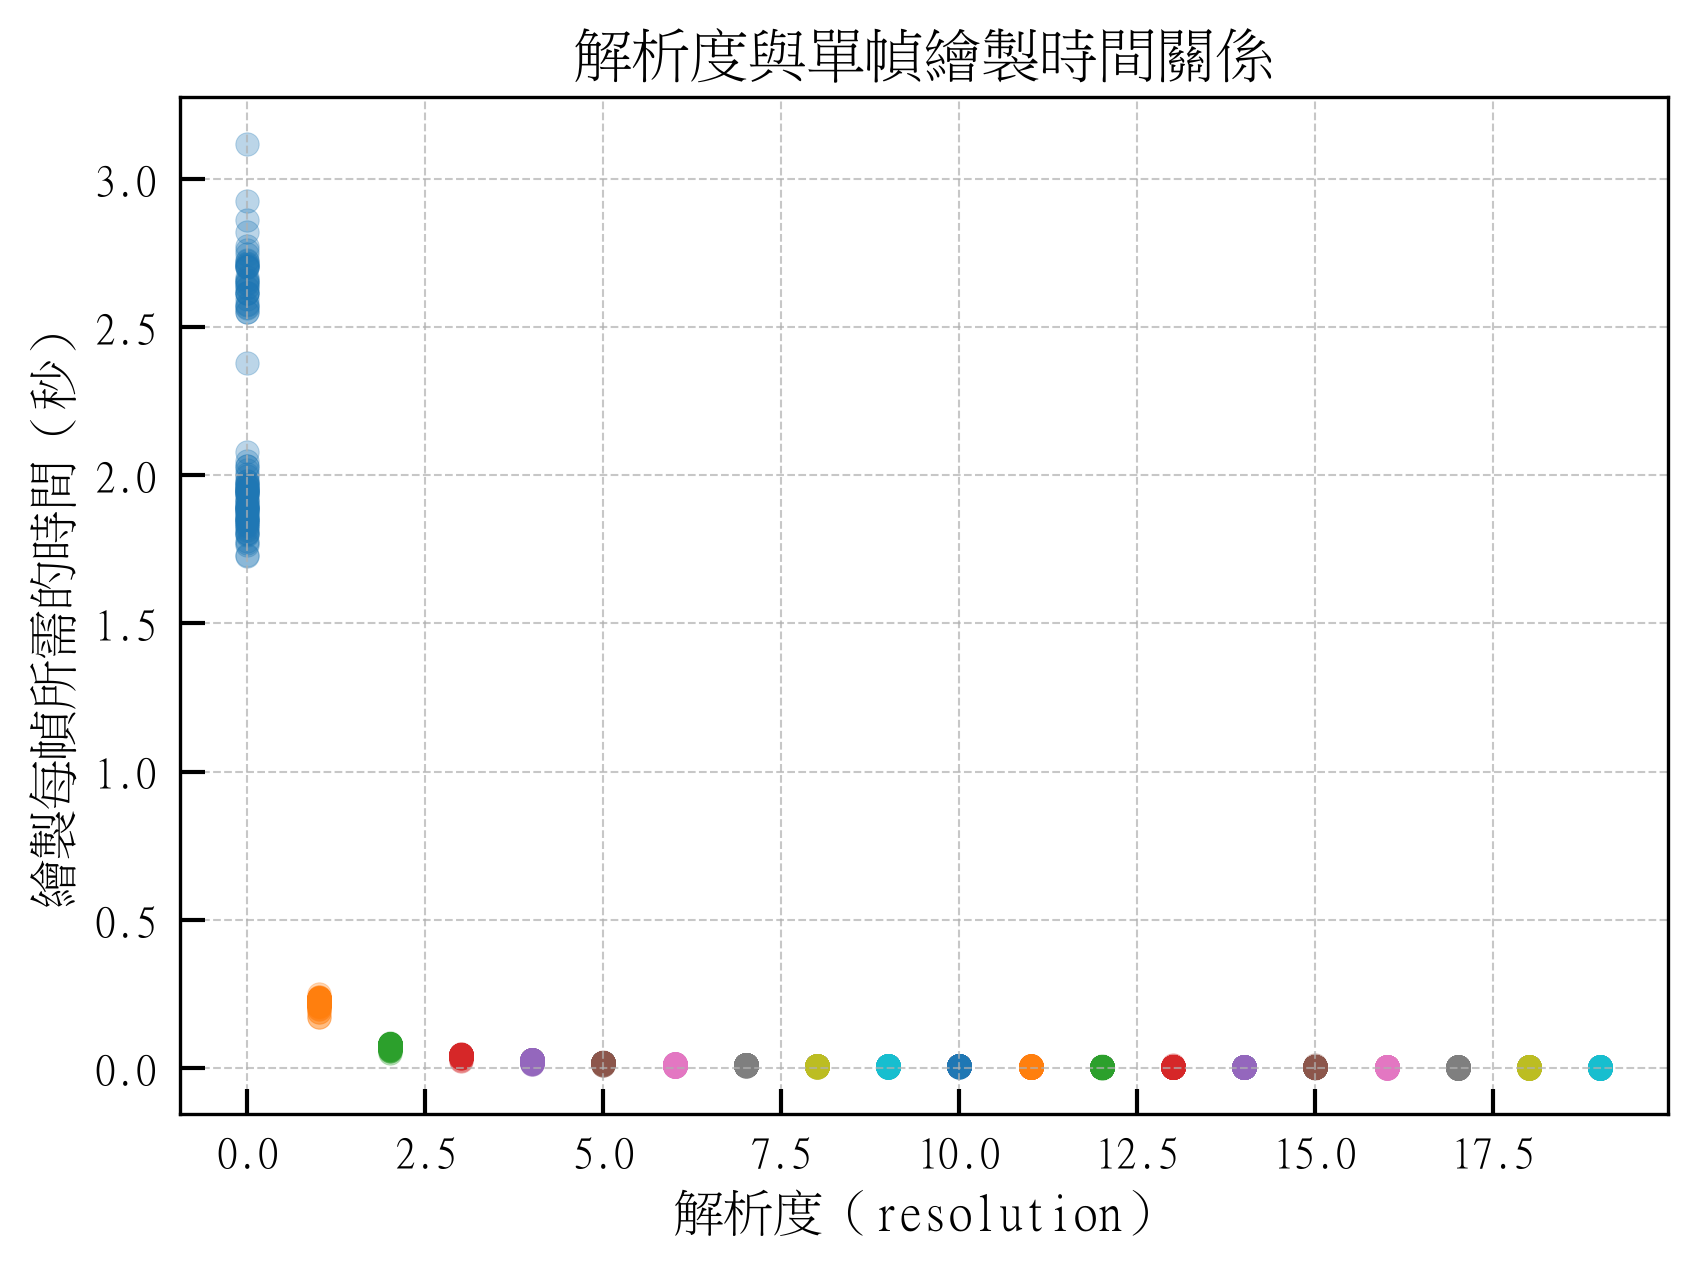
\includegraphics[width=\linewidth]{img/OutputImg/_Time_f-r.png} % 替換為你的圖片路徑
      \caption{線條長度與單幀繪製時間關係}
  \end{subfigure}

  \centering
  
  \caption{實驗一實驗結果}\label{fig:result_1}
\end{figure}

\newpage

\subsection{二、實驗二:各參數對數位鏡面顯示畫面的影響}

實驗二的結果如圖\ref{fig:result_2}、\ref{fig:result_3}與圖\ref{fig:result_4}(在下頁)。圖中的左中右分別為解析度、線條長度、寬度,顏色代表的是密度,即範圍內有多少組數據。另一方面,圖中,上面是達到穩定狀態所需的時間,下面則是穩定狀態與現實的差異,接下來將分別這兩點進行探討。

\begin{figure}[htbp]
  \centering
  \begin{subfigure}[b]{0.9\textwidth}
    \centering
    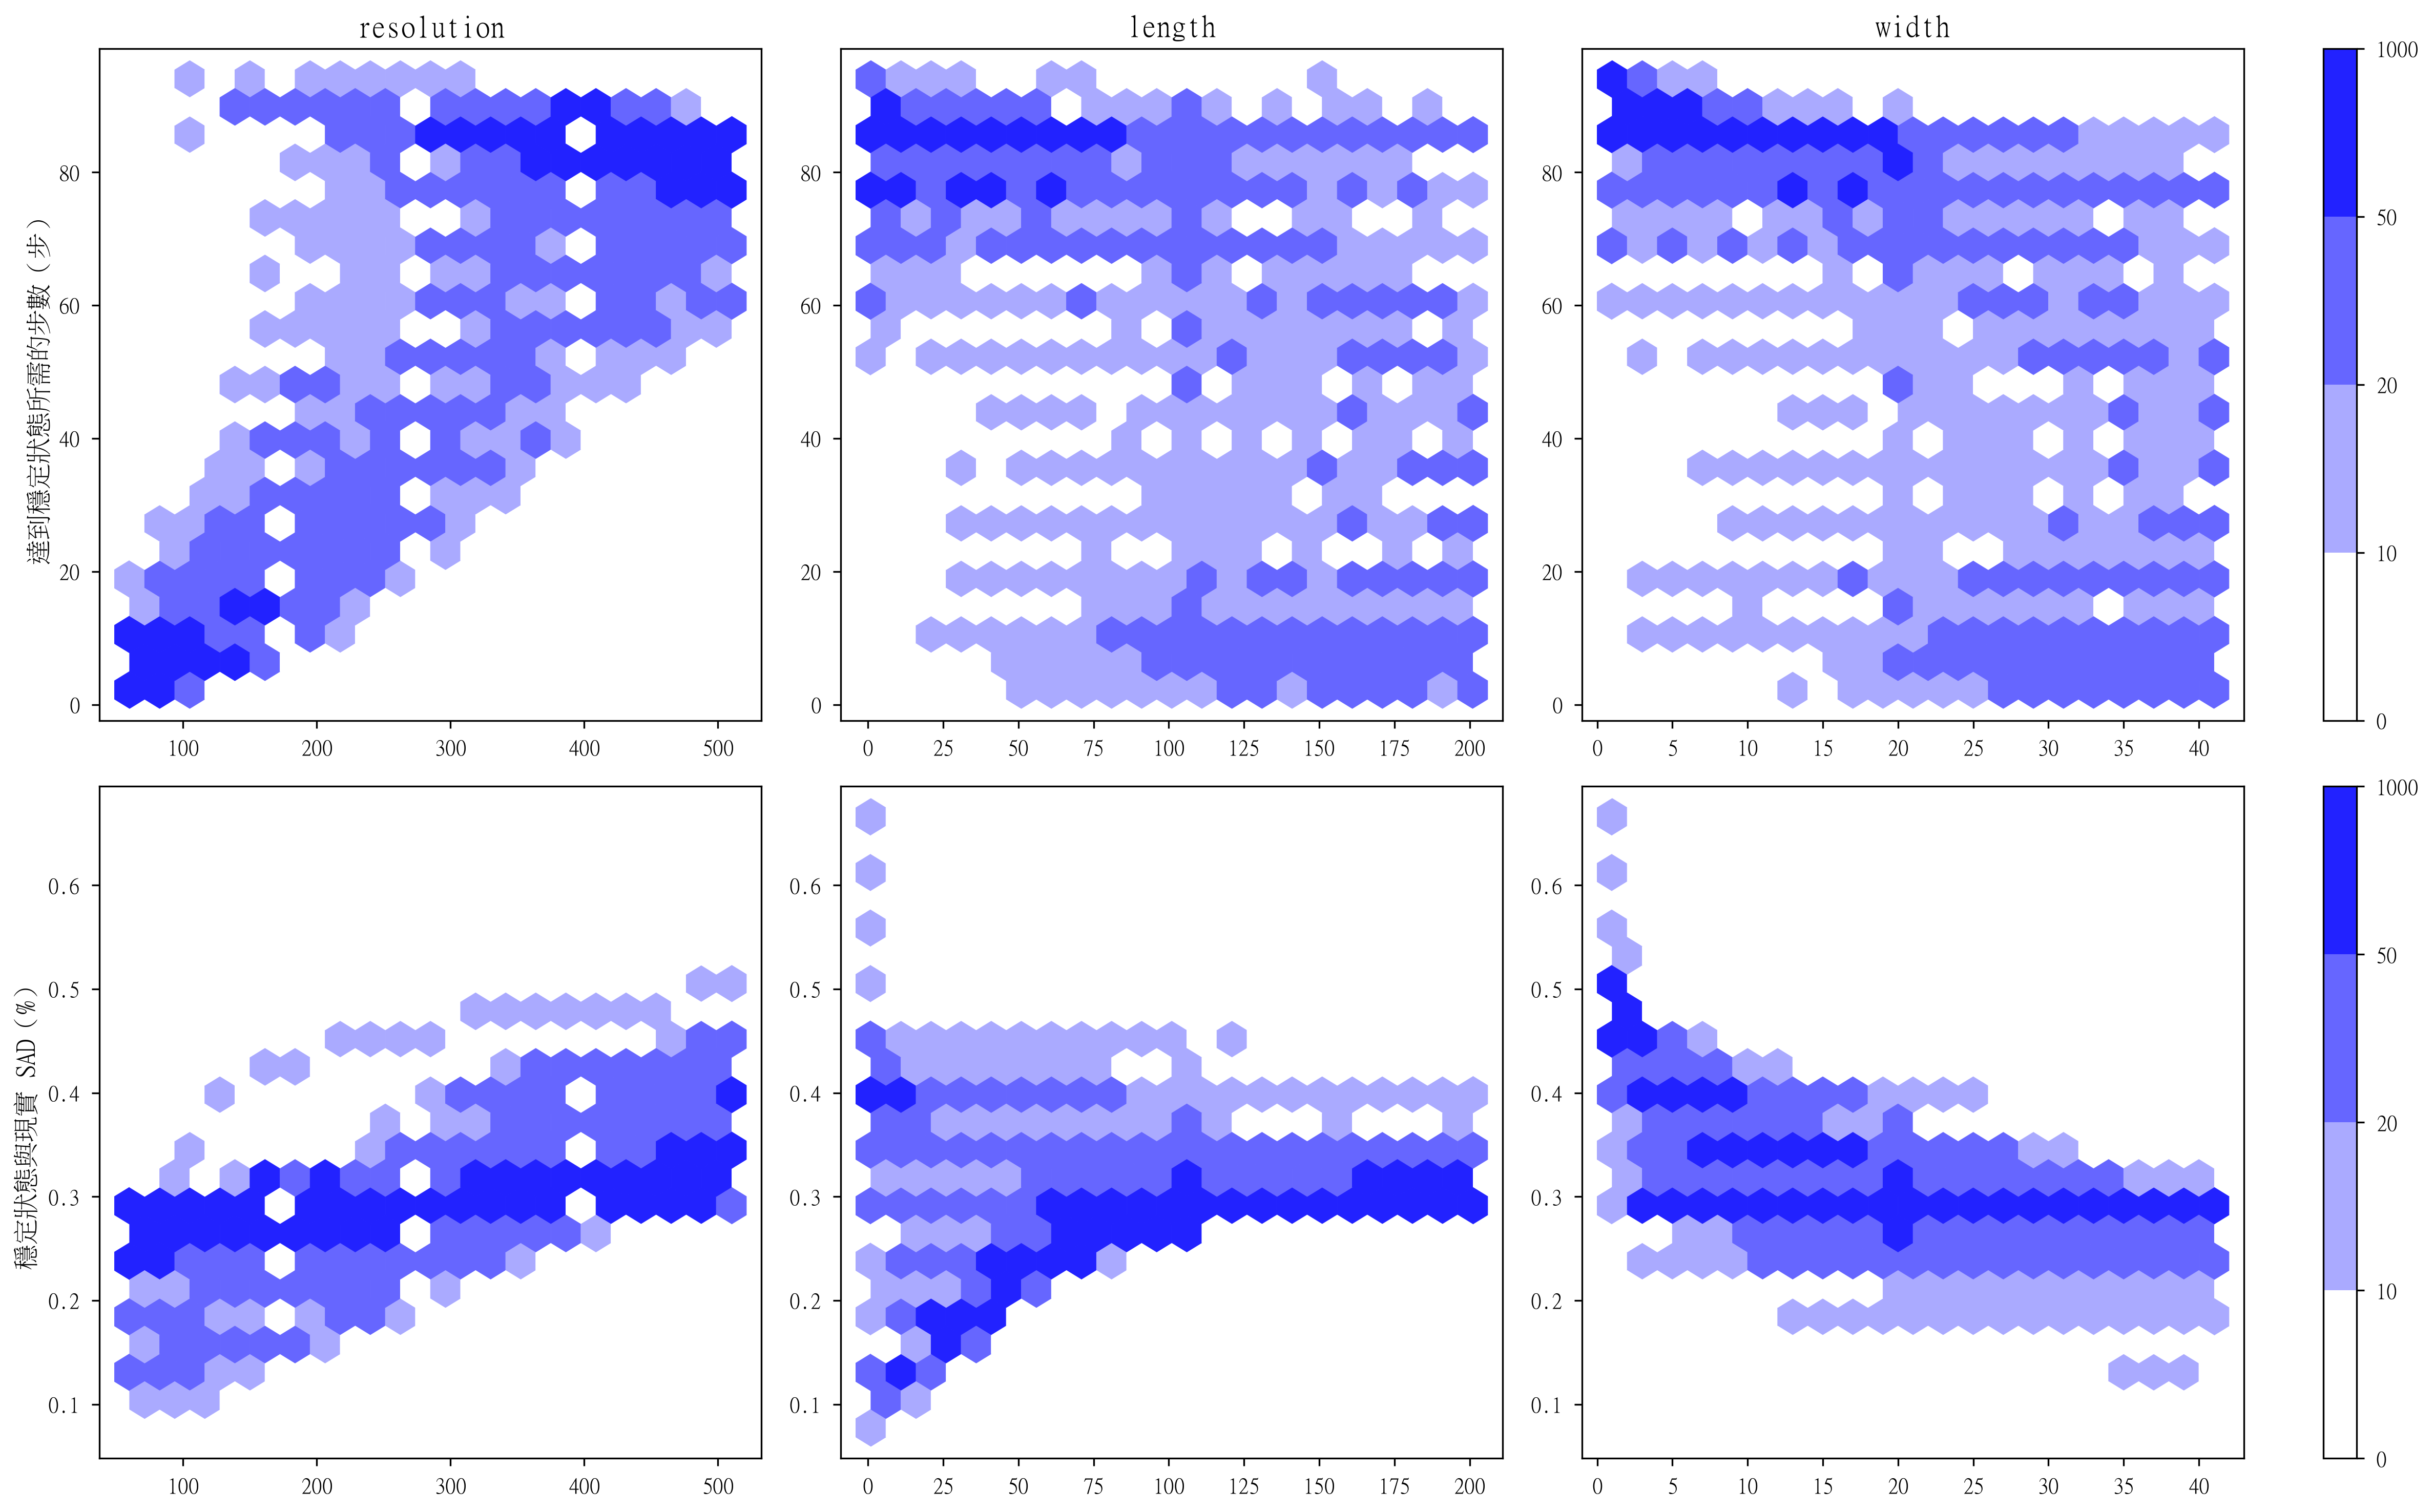
\includegraphics[width=\textwidth]{img/OutputImg/_Blank_BR.png}
    \caption{白藍交錯至紅黑交錯}
  \end{subfigure}

  \begin{subfigure}[b]{0.9\textwidth}
    \centering
    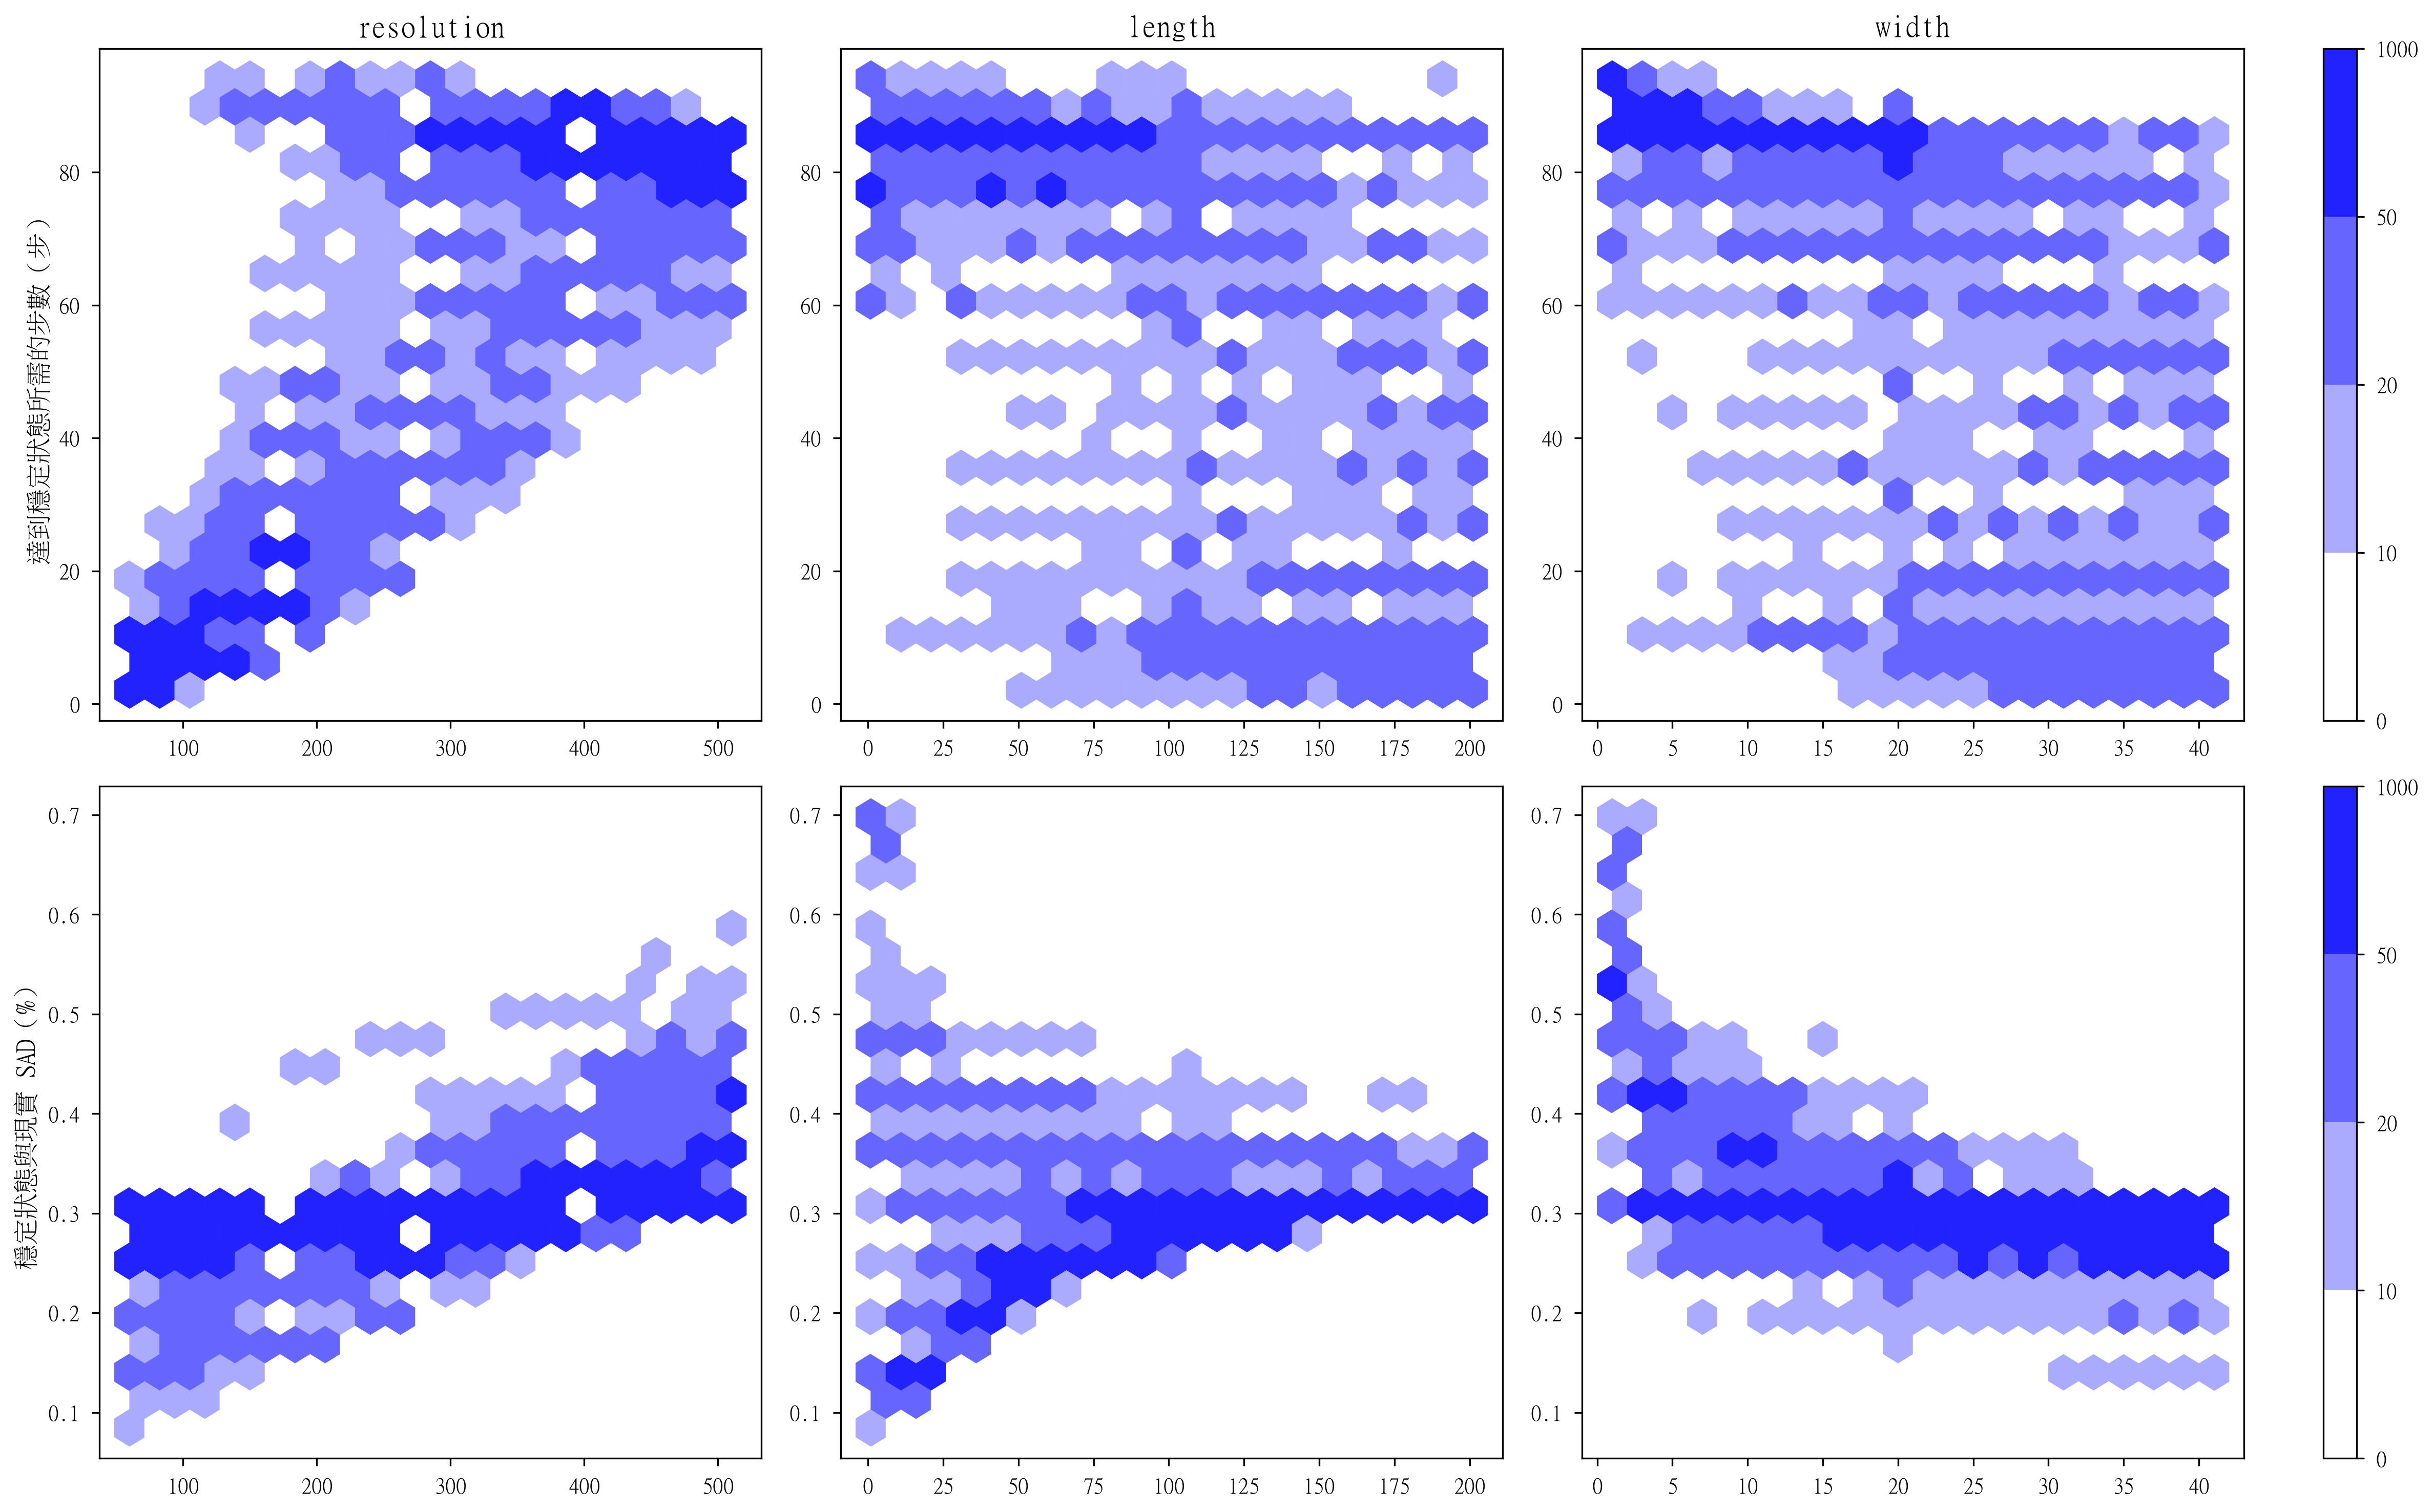
\includegraphics[width=\textwidth]{img/OutputImg/_Blank_BY.png}
    \caption{白藍交錯至黃黑交錯}
  \end{subfigure}

  \caption{實驗二實驗結果(一)}\label{fig:result_2}

\end{figure}

\begin{figure}[htbp]
  \centering
  \begin{subfigure}[b]{0.9\textwidth}
    \centering
    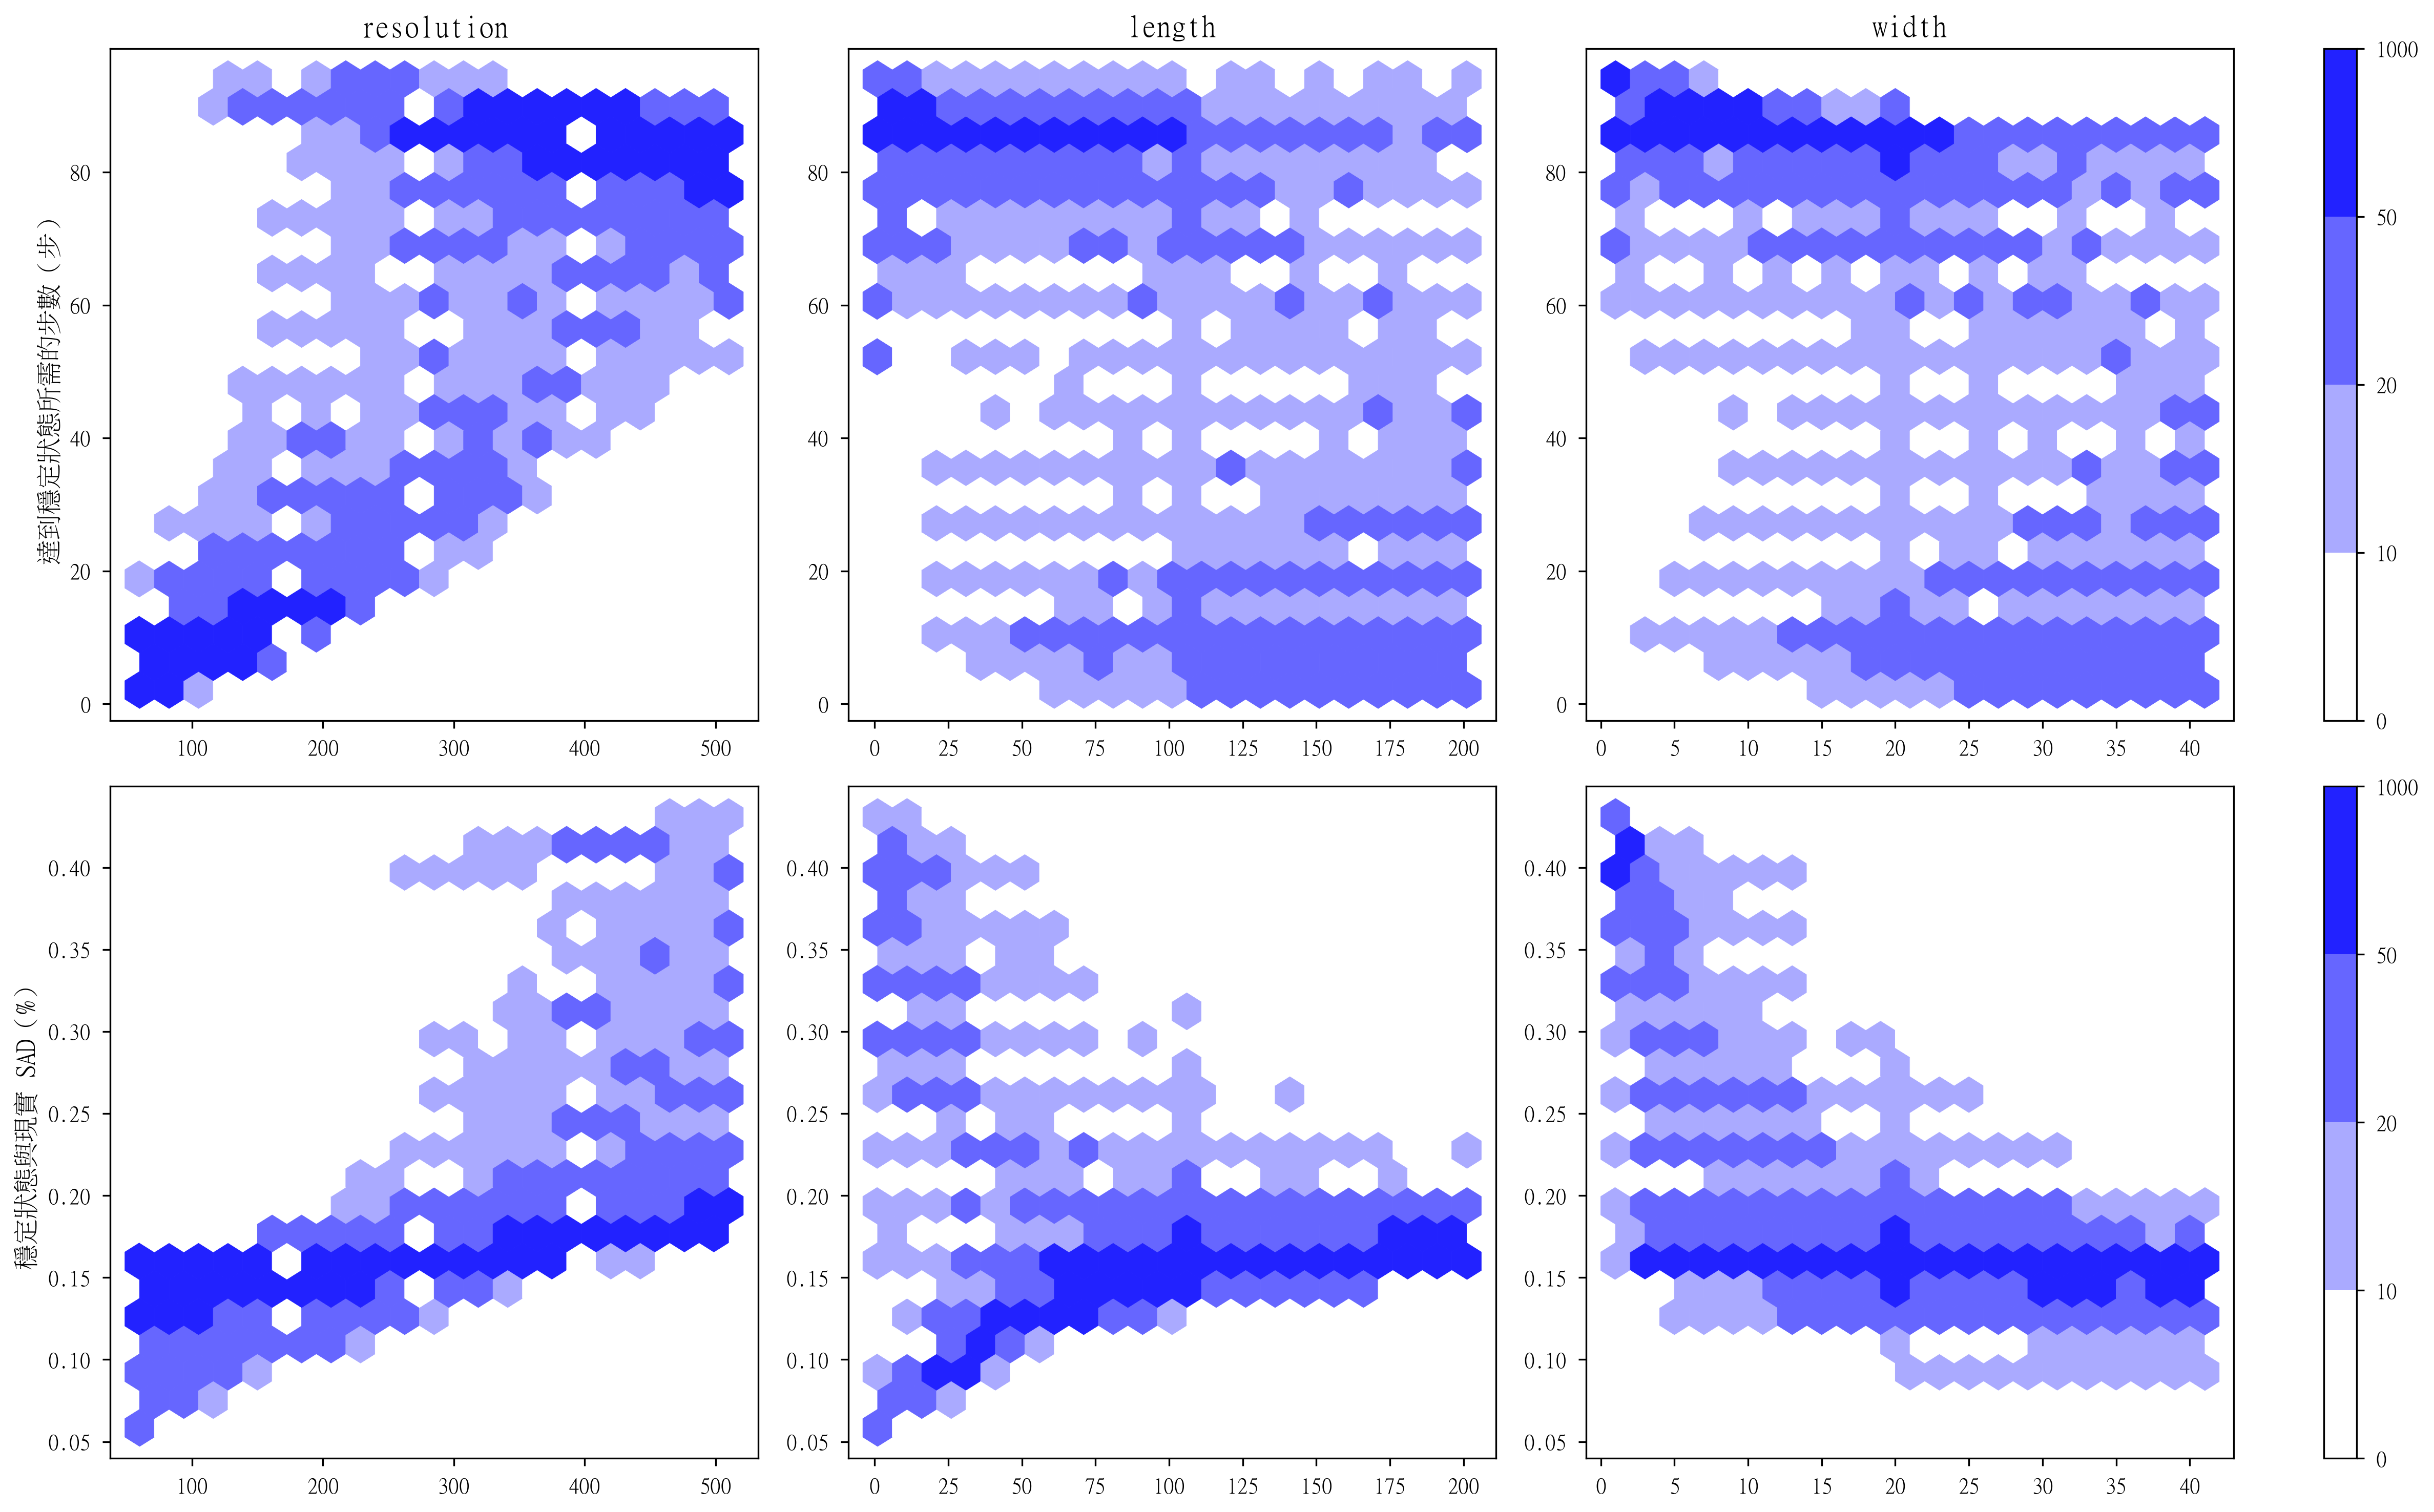
\includegraphics[width=\textwidth]{img/OutputImg/_Blank_RB.png}
    \caption{紅黑交錯至白藍交錯}
  \end{subfigure}

  \begin{subfigure}[b]{0.9\textwidth}
    \centering
    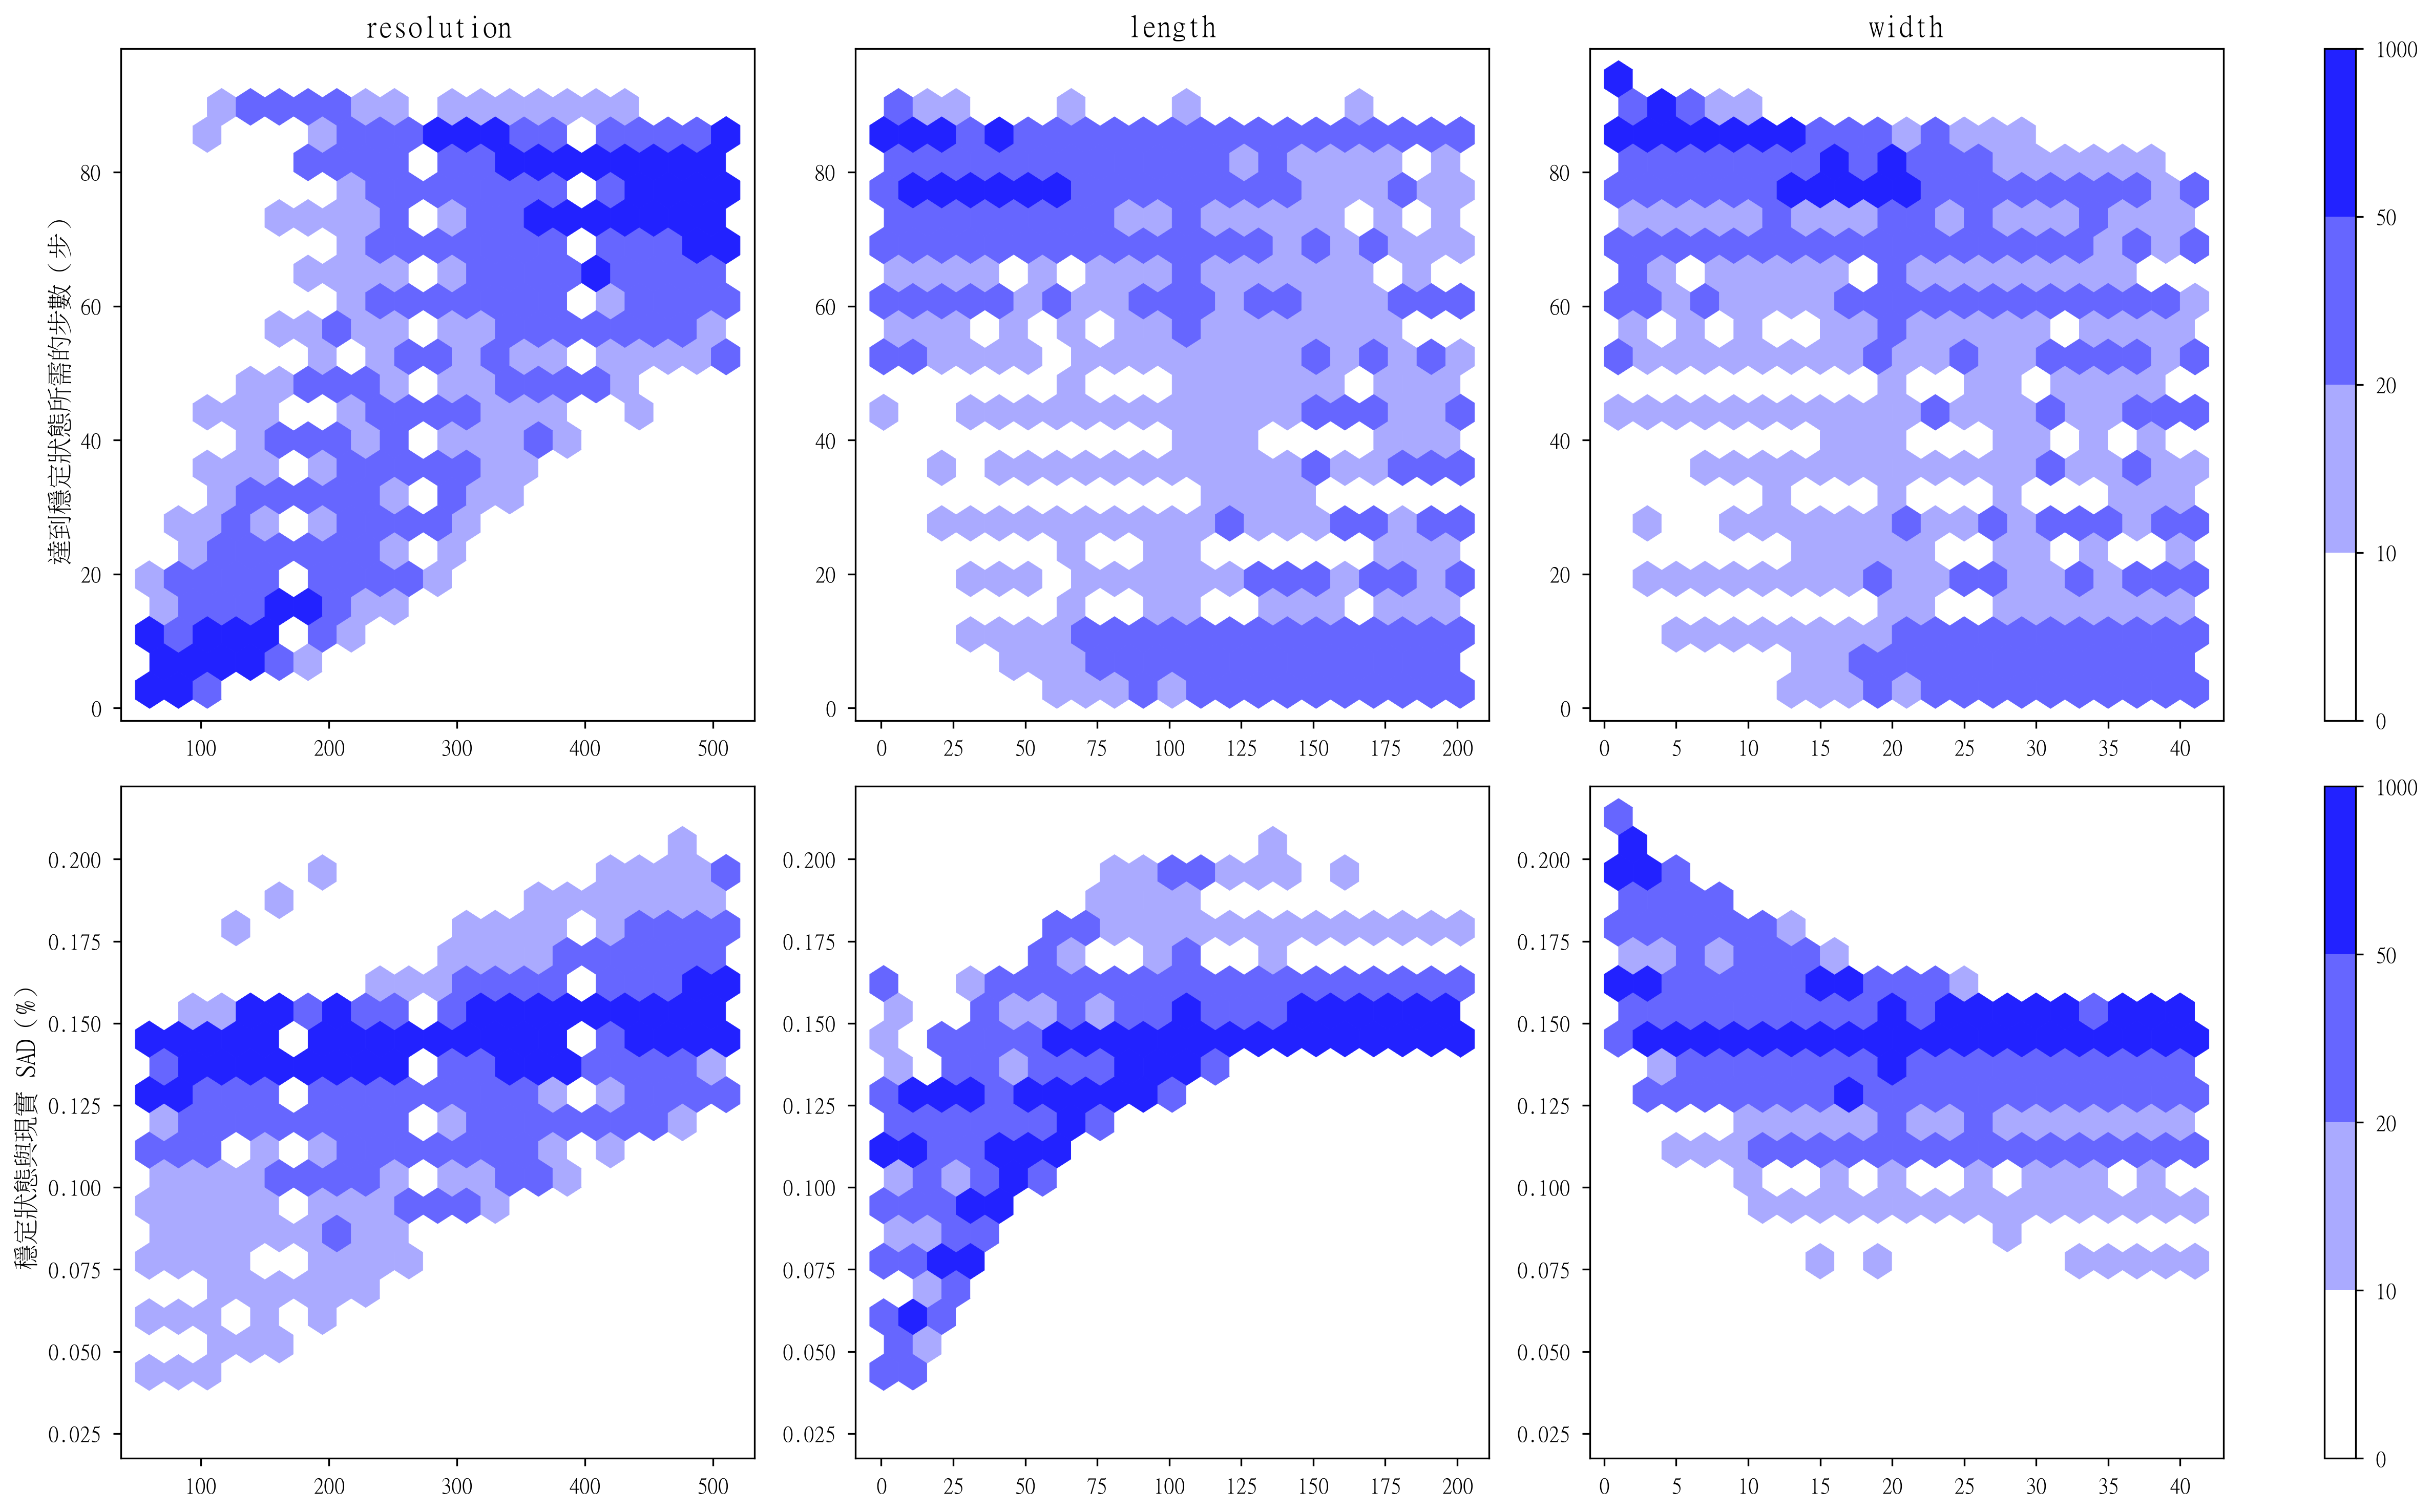
\includegraphics[width=\textwidth]{img/OutputImg/_Blank_RY.png}
    \caption{紅黑交錯至黃黑交錯}
  \end{subfigure}

  \caption{實驗二實驗結果(二)}\label{fig:result_3}

\end{figure}

\begin{figure}[htbp]
  \centering
  \begin{subfigure}[b]{0.9\textwidth}
    \centering
    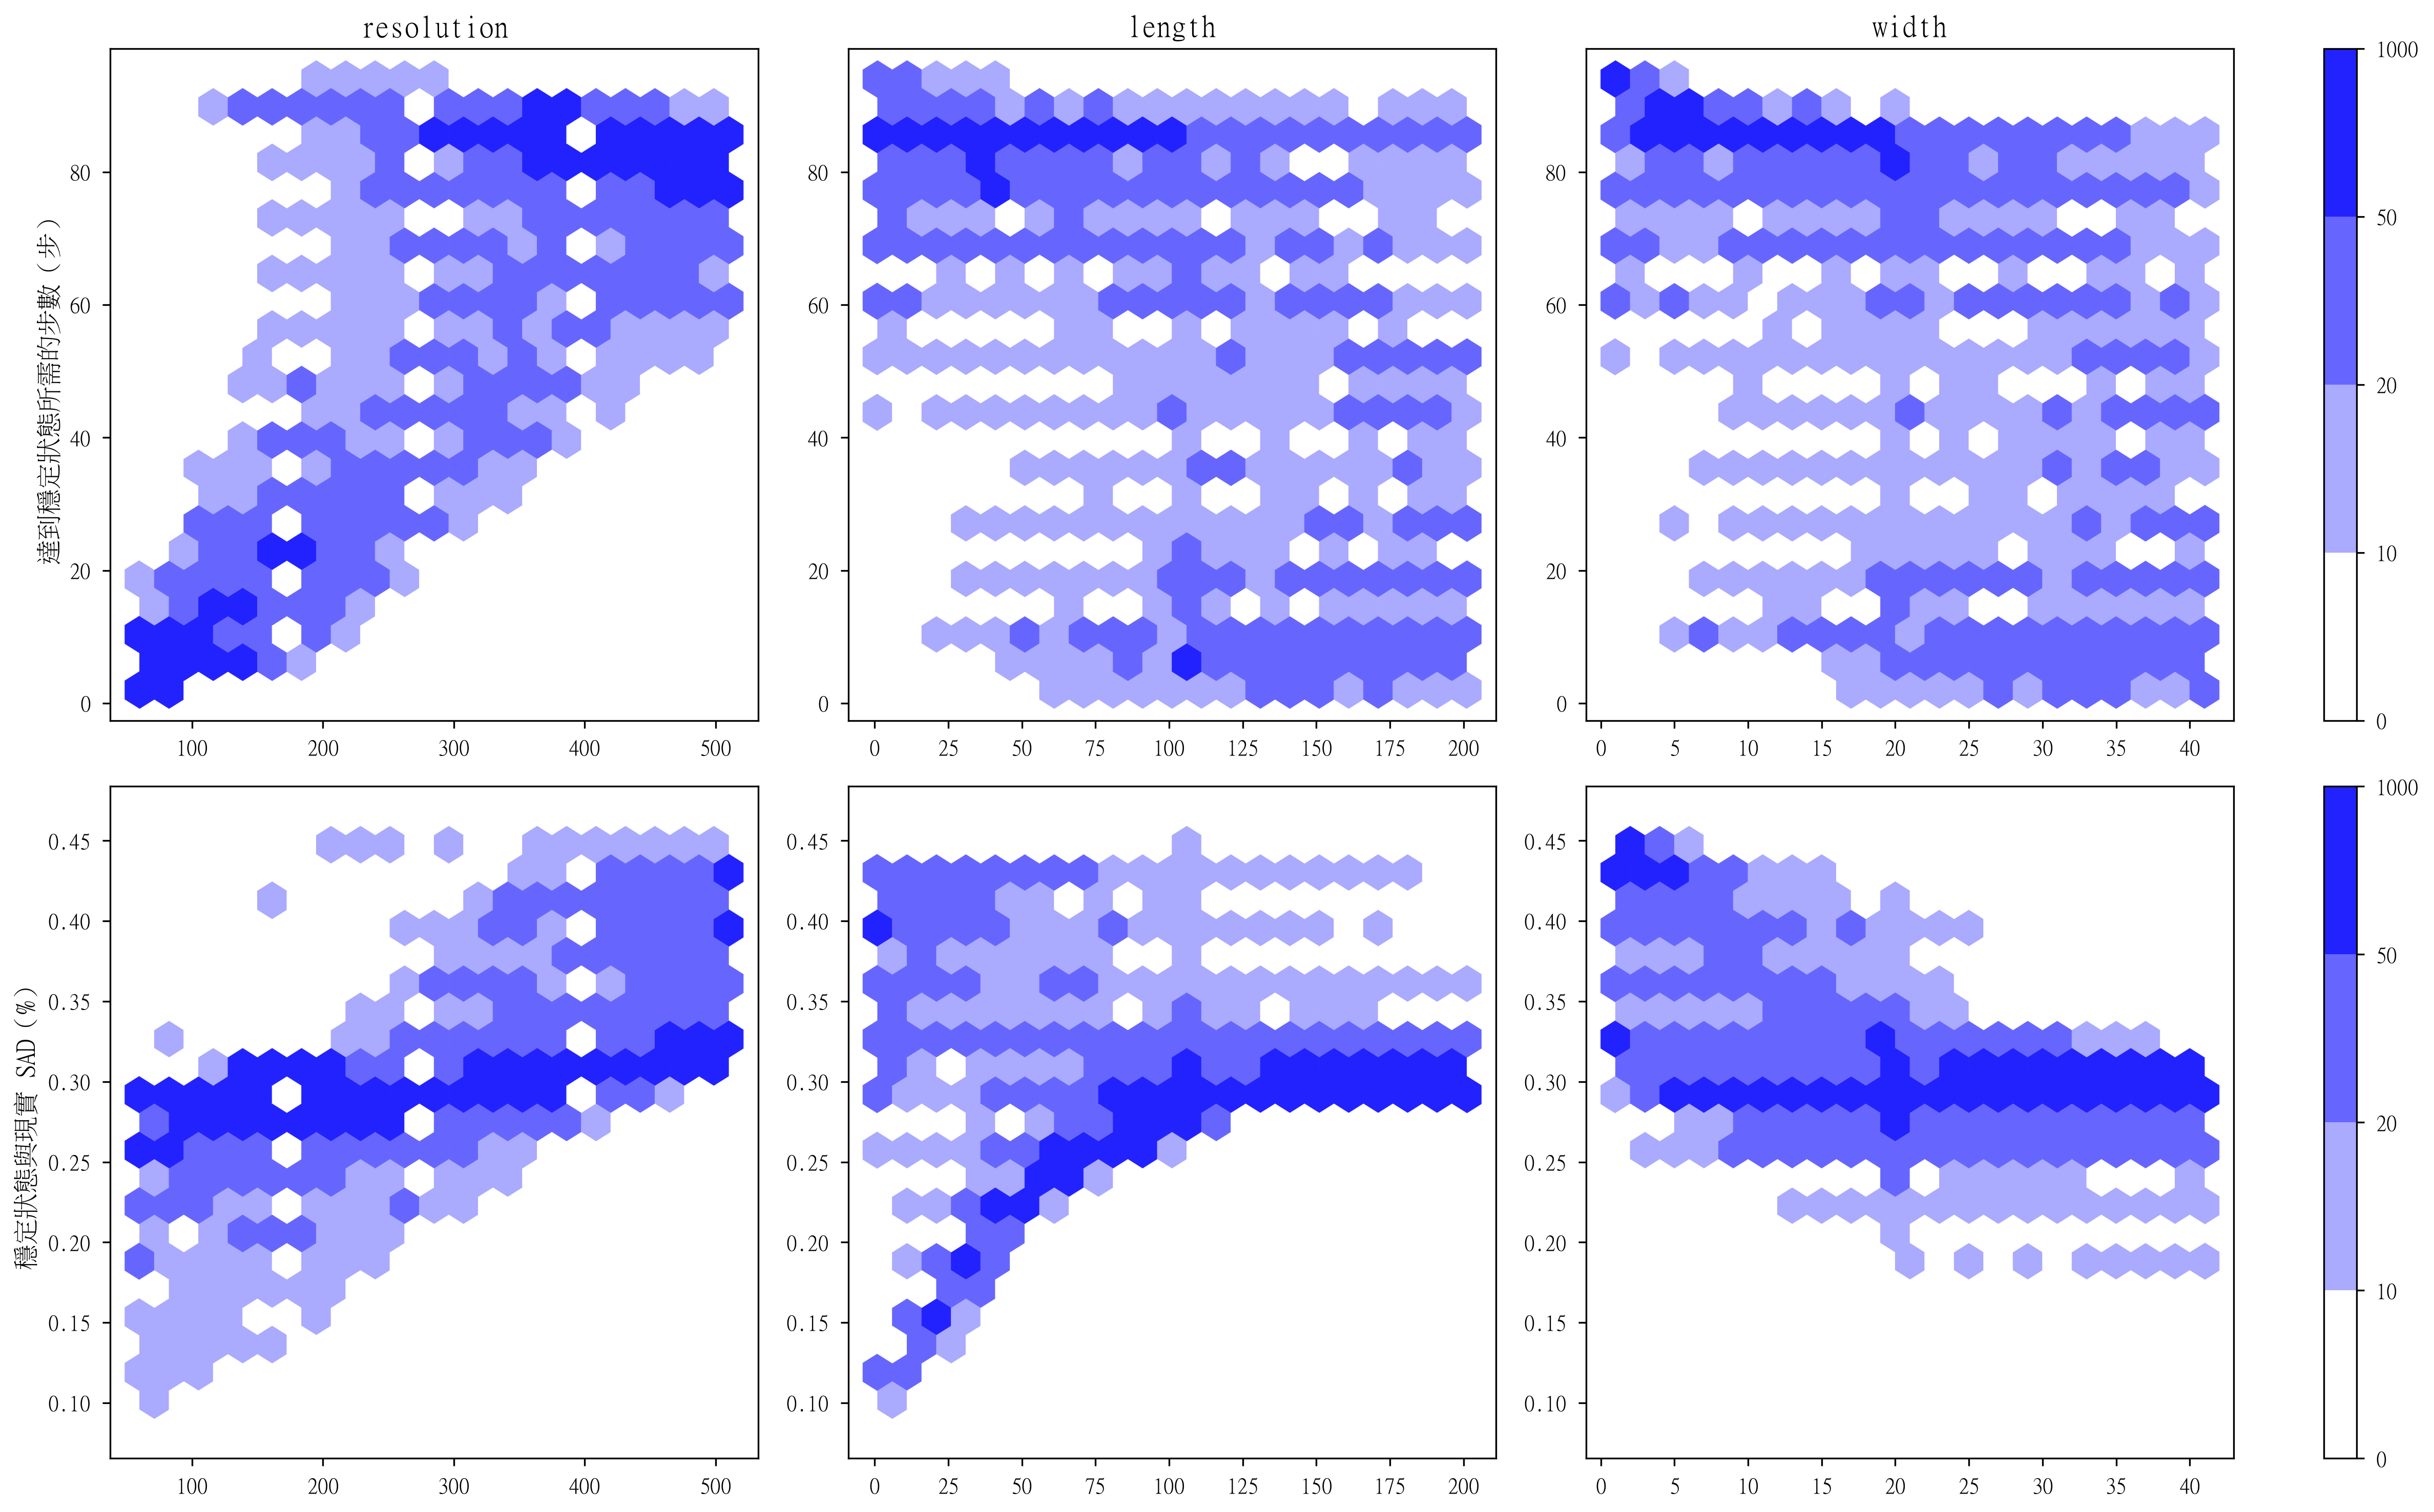
\includegraphics[width=\textwidth]{img/OutputImg/_Blank_YB.png}
    \caption{黃黑交錯至白藍交錯}
  \end{subfigure}

  \begin{subfigure}[b]{0.9\textwidth}
    \centering
    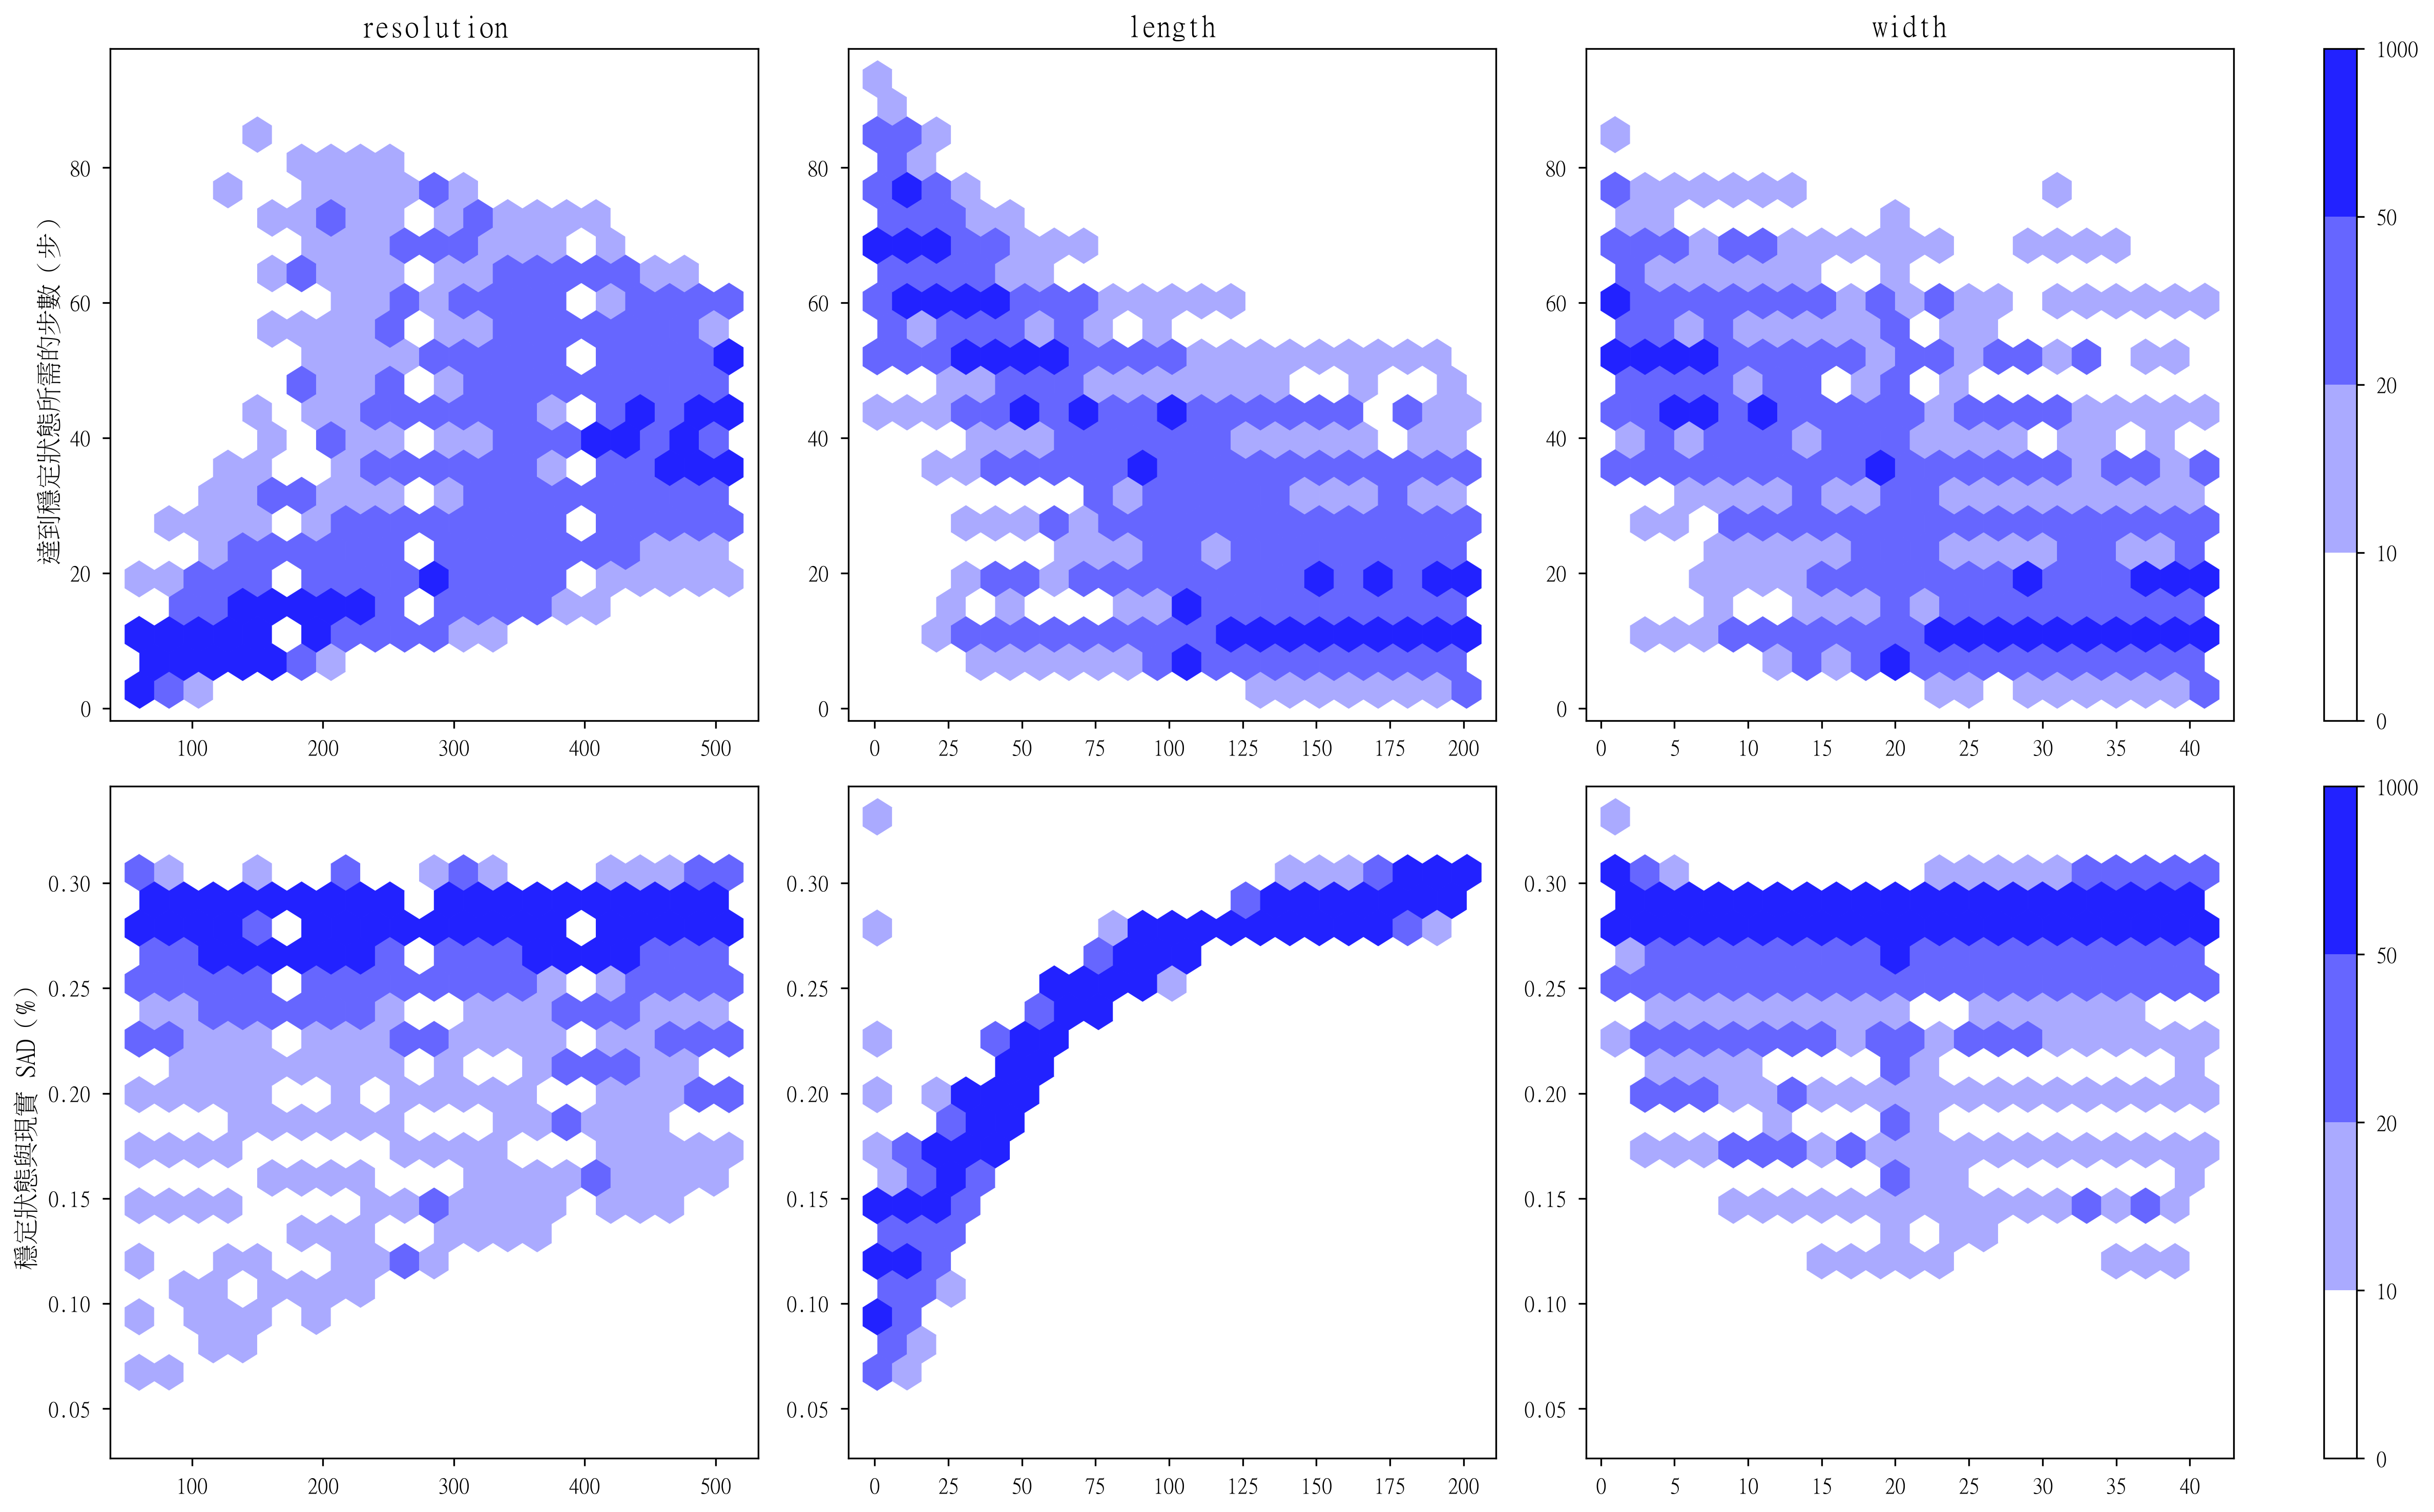
\includegraphics[width=\textwidth]{img/OutputImg/_Blank_YR.png}
    \caption{黃黑交錯至紅黑交錯}
  \end{subfigure}

  \caption{實驗二實驗結果(三)}\label{fig:result_4}

\end{figure}

\subsubsection{(一)達到穩定狀態所需的時間}

在達到穩定狀態所需的時間中,線條長度與線條寬度十分相似,皆呈現負相關,並且數據的形式類似斷層,即中間的過度數據少,左上與右下的數值多。而解析度則呈現正相關,也有類似斷層的現象,但比起線條長度與線條寬度較不明顯。

\subsubsection{(二)穩定狀態與現實的差異}

在穩定狀態與現實的差異中,線條長度呈現的特徵也與線條寬度類似,兩者在大多視情況中,數值低時會造成穩定狀態不穩定,但提高數值便會使其與現實的差異收斂到一定程度。

反觀解析度並沒有收斂這種現象,其無論數值大小,都會有一定的離群值。不過值得一提的是,在解析度上,一開始數值偏小時,離群值會偏低,而數值變大時,離群值則會上升,但收斂值卻不太會改變。

\newpage
\subsection{三、實驗三:不同場景對於數位鏡面的影響}

實驗結果如圖\ref{fig:result_5},我將其分為顏色數量與場景複雜程度來討論。就顏色數量而言,他們之間的差異程度並沒有決定性的差距,甚至對應不同組別也可能會有不同的結果。但在場景複雜度上,大多數狀況中,複雜程度高的場景明顯的比複雜程度低的場景SAD還要高。

而在2種顏色對應的複雜程度中由額外進行不同顏色的SAD實驗,在這之中,紅、綠、藍三色的SAD最低,再來是青、紫、黃,最高的是白。

\begin{figure}[htbp]
  \centering
  \begin{subfigure}[b]{0.9\textwidth}
    \centering
    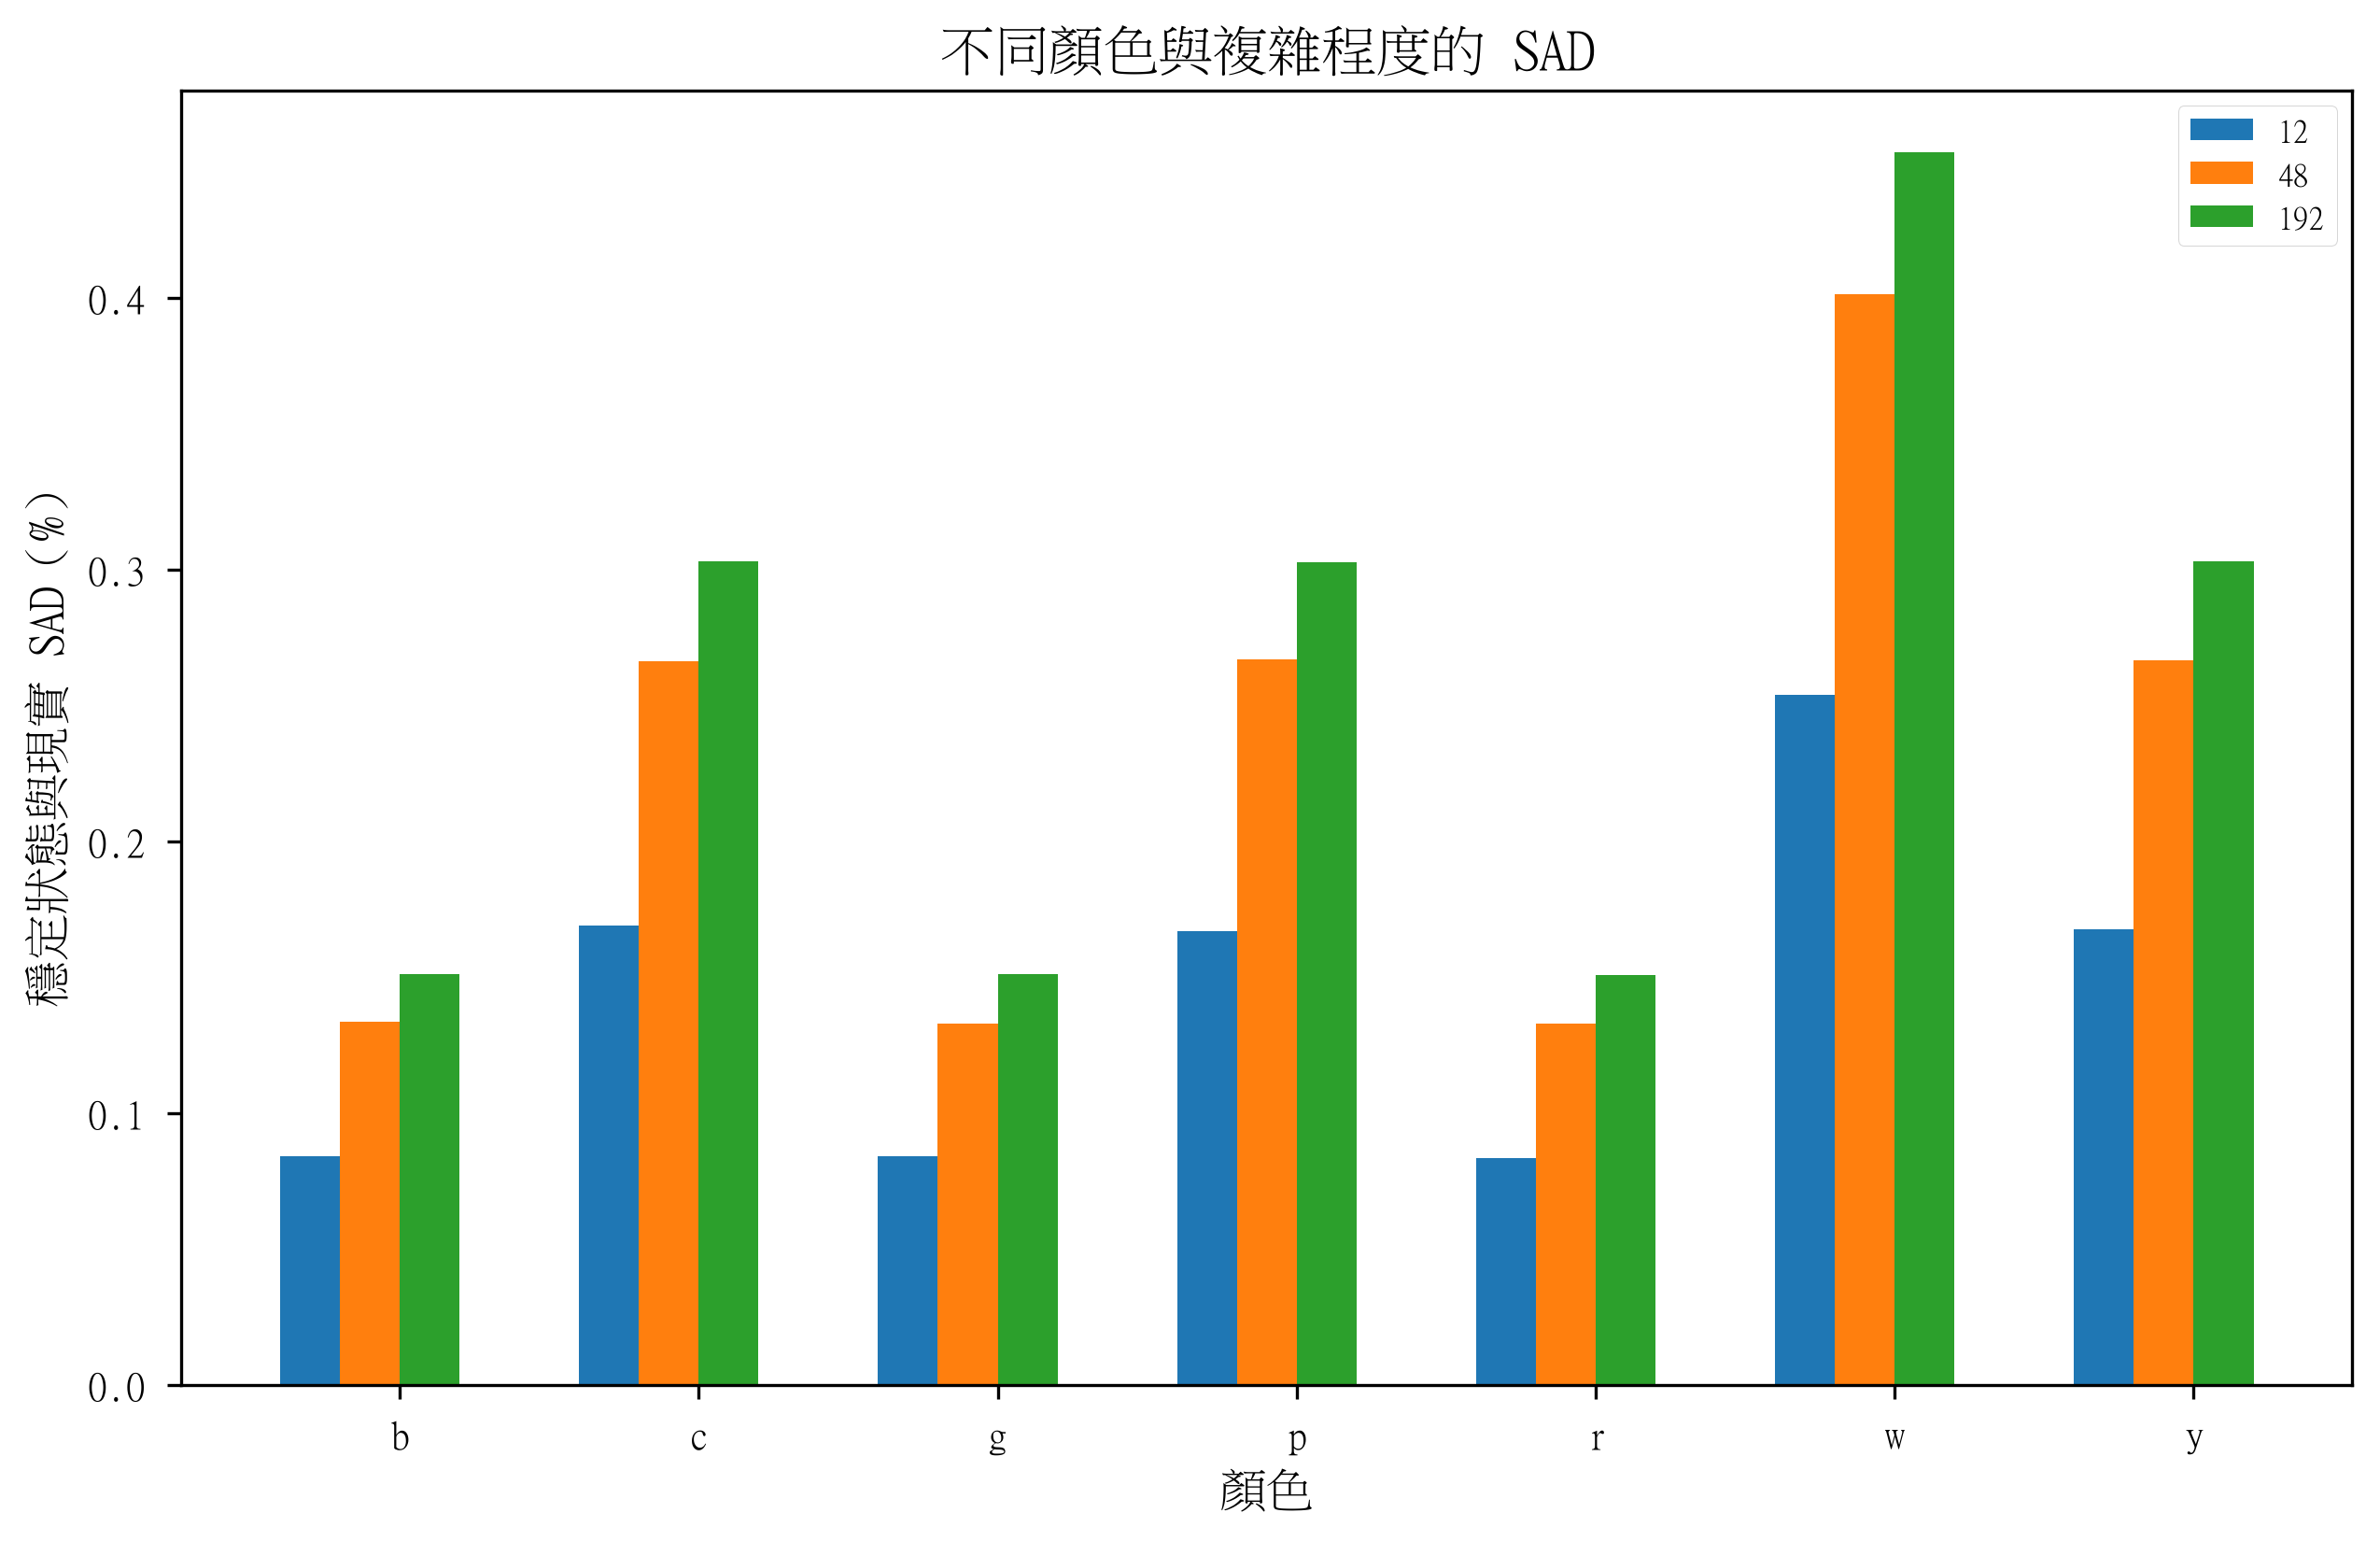
\includegraphics[width=\textwidth]{img/OutputImg/_Color_2.png}
    \caption{2 種顏色對應不同複雜程度}
  \end{subfigure}

  \begin{subfigure}[b]{0.45\textwidth}
    \centering
    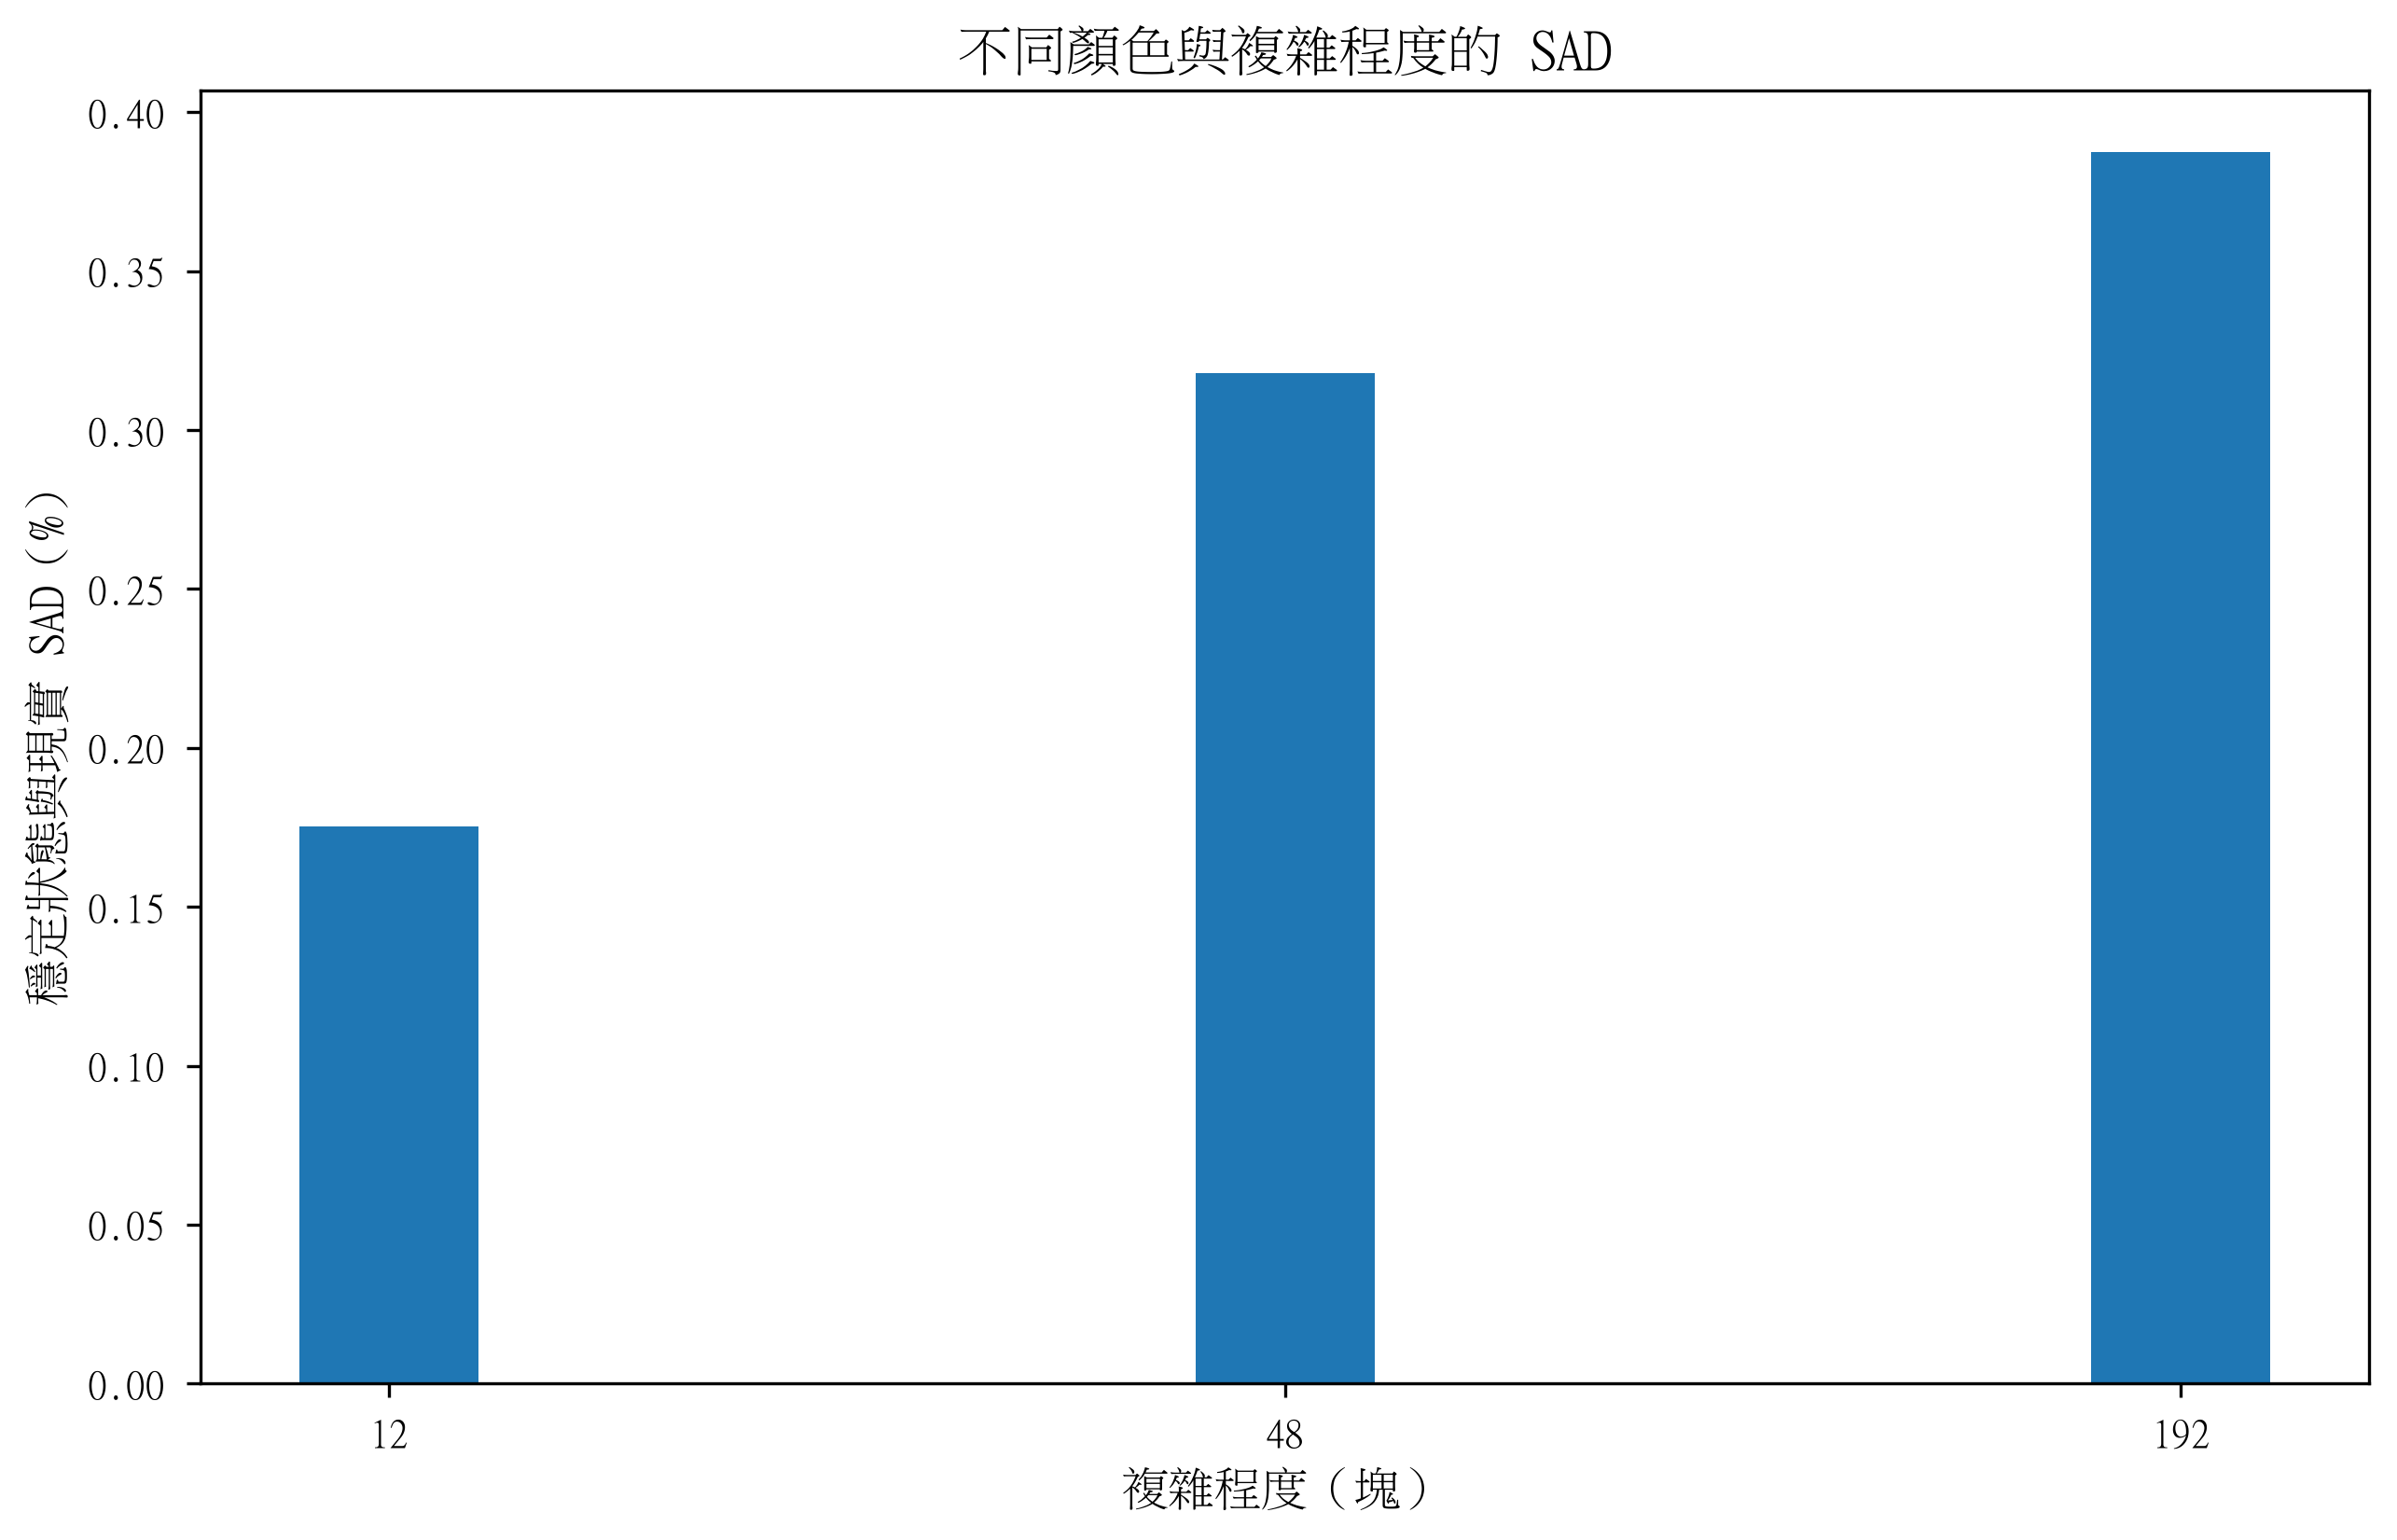
\includegraphics[width=\textwidth]{img/OutputImg/_Color_3.png}
    \caption{3 種顏色對應不同複雜程度}
  \end{subfigure}
  \begin{subfigure}[b]{0.45\textwidth}
    \centering
    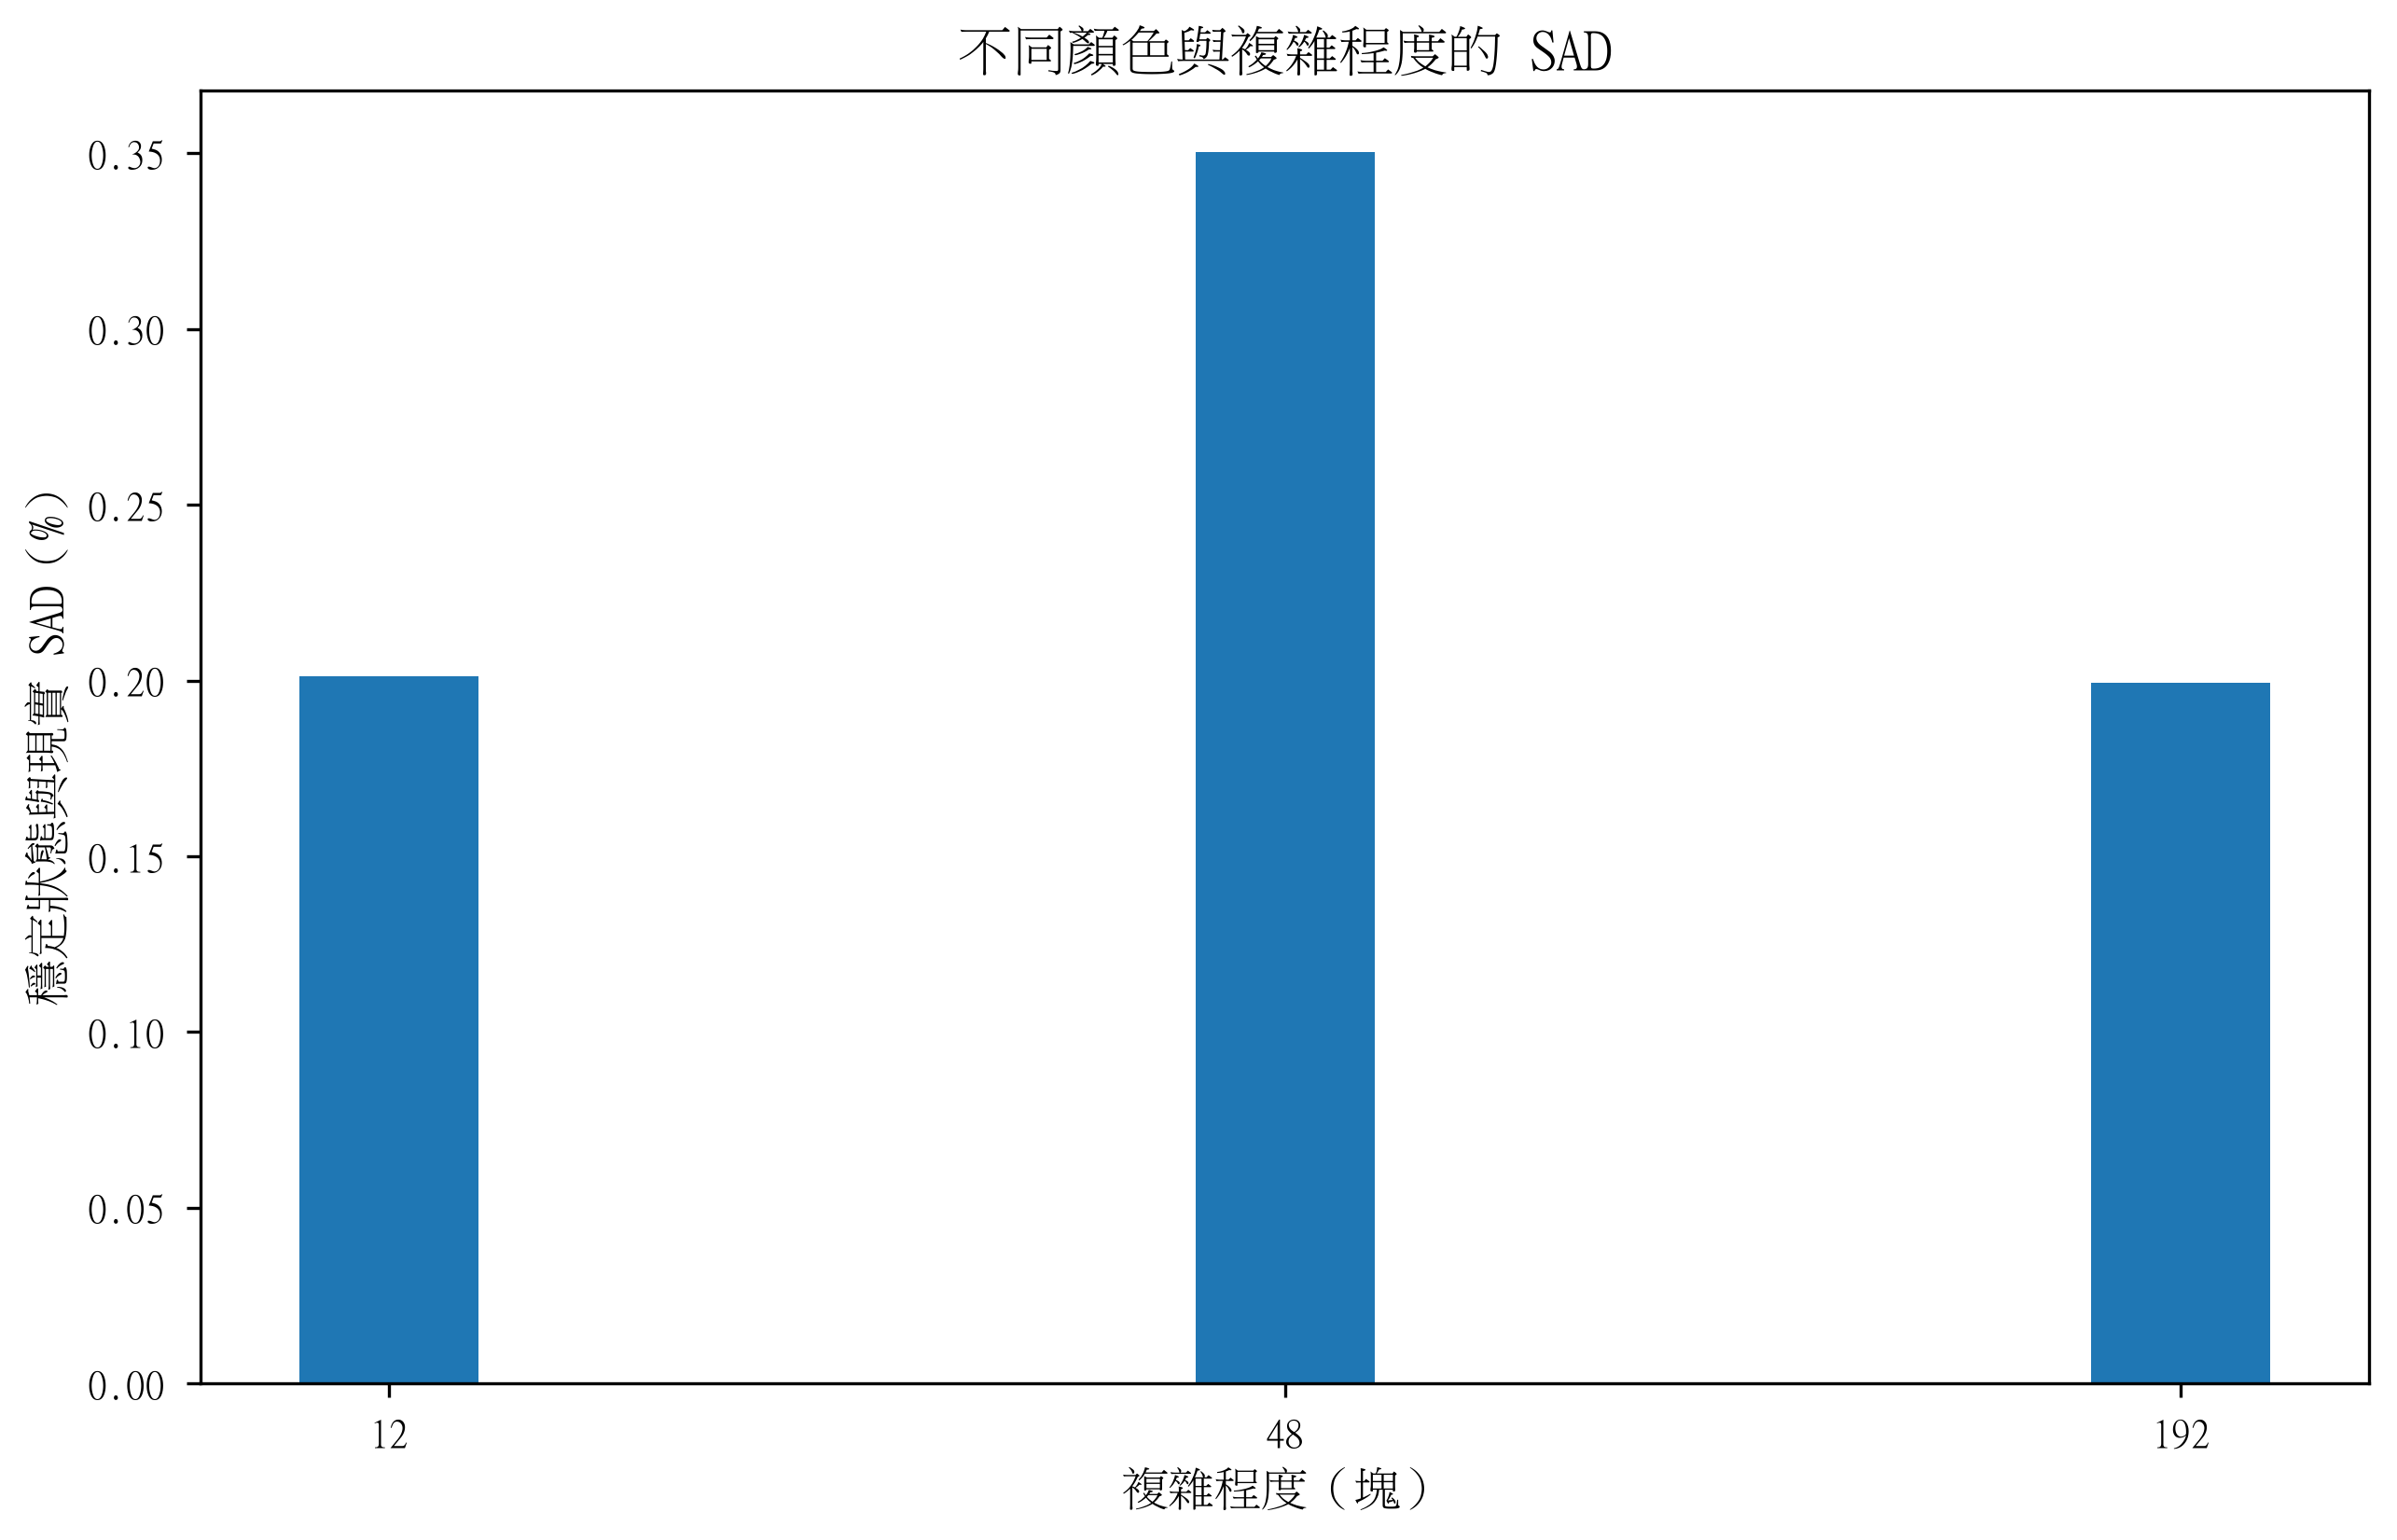
\includegraphics[width=\textwidth]{img/OutputImg/_Color_6.png}
    \caption{6 種顏色對應不同複雜程度}
  \end{subfigure}

  \caption{實驗三實驗結果}\label{fig:result_5}

\end{figure}

\newpage
\section{伍、討論}

\subsection{一、實驗一與時間複雜度}

若是對於數位鏡面進行時間複雜度的拆解可以寫出以下算式:

\[
O(\frac{l}{r^2}) 
\]

在算式中,$l$是指線條長度,$r$是指解析度,這兩項數值會對數位鏡面的執行時間造成最大的影響。其結果也大致符合實驗一的計算結果。唯一不符合的部分是在於線條長度對於單條線繪製時間的影響,我認為這是因為執行次數少,常數的影響大,因此時間複雜度的影響並不大,而當執行次數上升到繪製單幀時,其就呈現出了正向的相關。

\subsection{二、線條長度與線條寬度的相似}

在實驗二中,線條長度與線條寬度對於實驗結果的影響是類似的,我認為這是因為這兩項數值對於線條的影響類似,都是影響「線條的面積」,因此對於數位鏡面的影響相似。

\subsection{三、解析度的收斂值}

實驗二中,解析度一開始數值偏小時,離群值會偏低;數值變大時,離群值則會上升,但收斂值卻不太會改變。數位鏡面在當初設計時,解析度除了為了加速外,很大一部份想做的的事其實是減少隨機繪製造成的偏差(happpycorn,2024)。但在實驗結果中,解析度的限制其實只有對應到離群值,對於收斂值並沒有太多的影響,其中的原理或許是未來數位鏡面可以優化的契機。

\subsection{四、環境顏色與SAD}

在實驗三中,2種顏色對應的複雜程度額外進行的不同顏色SAD實驗中,紅、綠、藍三色的SAD最低,再來是青、紫、黃,最高的是白。我發現其數值某種程度上與他對應的另一個顏色(黑)的SAD呈現正相關,這表示環境在一定程度上對於數位鏡面呈現的效果是有影響的。我認為要對數位鏡面進行優化的話,或許可以針對不同的環境進行優化。

\subsection{五、數位鏡面的最優設定}

由於藝術並沒有所謂的最優解,這裡主要探討的是對應的需求下會需要的不同參數設定。若是希望反應的速度慢些,有點變化的感覺,可以調低線條的長度、寬度,調高解析度,反之亦然。若是希望更貼合現實的畫面的話,可以調低解析度。若是希望畫面的隨機性增加,則可以減少線條的長度與寬度。

\newpage
\section{陸、結論}

\subsubsection{(一)了解不同參數設定對於數位鏡面的影響}

在執行時間方面,線條寬度不相關、線條長度呈正相關、解析度呈負指數相關。達到穩定狀態所需的時間方面,解析度呈正相關、線條寬度與線條長度呈負相關。穩定狀態與現實的差異方面,線條寬度與線條長度在數值低時不穩定、數值高時則會收斂;解析度無論高低收斂值都類似,但離群值在數值低時偏低、在數值高時偏高。

\subsubsection{(二)了解不同影像環境對於數位鏡面的影響}

在環境複雜度方面,複雜度越高、相同設定下的與現實差異就會越大;顏色數量對於相同設定下的與現實差異影響並不大。

在2種顏色做的額外實驗中,2種顏色的差異越大、畫面與現實的差異越大。

\subsubsection{(三)探討不同環境與需求下數位鏡面的最優設定}

若希望反應較慢且有些變化,可降低線條長度與寬度,提升解析度;反之,增長線條並降低解析度可加快反應速度。為貼近現實,可降低解析度;增加隨機性則可縮短線條並減小寬度。

\newpage
\section{柒、參考文獻資料}

% \noindent
% \href{https://www.husart.net/?p=372}{丹尼爾羅森的數位鏡面} \\

% \noindent
% \href{https://github.com/happpycorn/Mirror_Line}{我的數位鏡面}

\end{document}